\documentclass[12pt]{article}
\renewcommand{\baselinestretch}{1}
\usepackage[left=3cm,bottom=3cm,right=3cm,top=3cm]{geometry}

%% Packages
\usepackage{amsmath,amsfonts}
\usepackage{array}
\usepackage[caption=false,font=normalsize,labelfont=sf,textfont=sf]{subfig}
\usepackage{textcomp}
\usepackage{stfloats}
\usepackage{url}
\usepackage{verbatim}
\usepackage{graphicx}
\usepackage{mathtools}
\usepackage{algorithm}
\usepackage{algorithmic}
\usepackage{cases}
\usepackage{enumerate}
\usepackage{tabularx}
\usepackage{multirow}
\usepackage{bm}
\usepackage{algorithm}
\usepackage{authblk}
\usepackage{algorithmic}
\usepackage{indentfirst}
\usepackage{setspace}
\usepackage{color}
\usepackage[utf8]{inputenc} % allow utf-8 input
\usepackage[T1]{fontenc}    % use 8-bit T1 fonts
\usepackage{hyperref}       % hyperlinks
\usepackage{url}            % simple URL typesetting
\usepackage{booktabs}       % professional-quality tables
\usepackage{amsfonts}       % blackboard math symbols
\usepackage{nicefrac}       % compact symbols for 1/2, etc.
\usepackage{microtype}      % microtypography
\usepackage{lipsum}		% Can be removed after putting your text content
\usepackage{graphicx}
\usepackage{doi}
\usepackage{amssymb}                  
\usepackage{mathrsfs} 
\usepackage[resetlabels]{multibib}
\usepackage[bottom]{footmisc}
\newtheorem{definition}{Definition}
\newtheorem{lemma}{Lemma}
\newtheorem{theorem}{Theorem}
\newtheorem{corollary}{Corollary}
\newtheorem{proof}{Proof}
\newtheorem{remark}{Remark}
\newtheorem{assumption}{Assumption}
\providecommand{\keywords}[1]{\textit{\quad Key words }:  #1}
\newcommand*{\QEDB}{\null\nobreak\hfill\ensuremath{\square}}
\hyphenation{op-tical net-works semi-conduc-tor IEEE-Xplore}
% updated with editorial comments 8/9/2021
\usepackage[utf8]{inputenc}
\usepackage{natbib}
\renewcommand{\algorithmicrequire}{ \textbf{Input:}}
\renewcommand{\algorithmicensure}{ \textbf{Output:}} 
\usepackage{tikz}
\usetikzlibrary{patterns}
\usetikzlibrary{decorations.pathreplacing,calligraphy}
\usetikzlibrary{patterns.meta}
\usetikzlibrary{arrows.meta}
\tikzdeclarepattern{
  name=mylines,
  parameters={
      \pgfkeysvalueof{/pgf/pattern keys/size},
      \pgfkeysvalueof{/pgf/pattern keys/angle},
      \pgfkeysvalueof{/pgf/pattern keys/line width},
      \pgfkeysvalueof{/pgf/pattern keys/pat},
  },
  bounding box={
    (0,-0.5*\pgfkeysvalueof{/pgf/pattern keys/line width}) and
    (\pgfkeysvalueof{/pgf/pattern keys/size},
0.5*\pgfkeysvalueof{/pgf/pattern keys/line width})},
  tile size={(\pgfkeysvalueof{/pgf/pattern keys/size},
\pgfkeysvalueof{/pgf/pattern keys/size})},
  tile transformation={rotate=\pgfkeysvalueof{/pgf/pattern keys/angle}},
  defaults={
    size/.initial=5pt,
    angle/.initial=45,
    line width/.initial=.4pt,
    pat/.initial=dashed,
  },
  code={
      \draw [line width=\pgfkeysvalueof{/pgf/pattern keys/line width},\pgfkeysvalueof{/pgf/pattern keys/pat}]
        (0,0) -- (\pgfkeysvalueof{/pgf/pattern keys/size},0);
  },
}
%\setcitestyle{numbers}


\usepackage{graphicx} % Required for inserting images



\begin{document}


\title{Exact recovery in the double sparse model: sufficient and necessary signal conditions}

\author[1]{Shixiang Liu}
\author[2]{Zhifan Li}
\author[1]{Yanhang Zhang}
\author[1, 3]{Jianxin Yin}

\affil[1]{\footnotesize School of Statistics, Renmin University of China}
\affil[2]{\footnotesize Beijing Institute of Mathematical Sciences and Applications}
\affil[3]{\footnotesize Center for Applied Statistics and School of Statistics, Renmin University of China}

\date{}
\maketitle \sloppy

\begin{abstract}
The double sparse linear model, which has both group-wise and element-wise sparsity in regression coefficients, has attracted lots of attention recently. 
This paper establishes the sufficient and necessary relationship between the exact support recovery and the optimal minimum signal conditions in the double sparse model. 
Specifically, sharply under the proposed signal conditions, a two-stage double sparse iterative hard thresholding procedure achieves exact support recovery with a suitably chosen threshold parameter.
Also, this procedure maintains asymptotic normality aligning with an OLS estimator given true support, hence holding the oracle properties.
Conversely, we prove that no method can achieve exact support recovery if these signal conditions are violated. 
This fills a critical gap in the minimax optimality theory on support recovery of the double sparse model.
Finally, numerical experiments are provided to support our theoretical findings.
\end{abstract}

\begin{keywords}
 {Double sparse}, {Exact recovery}, {Minimax optimality}, {Oracle properties}, {Variable selection}
\end{keywords}

 

\section{Introduction}\label{sec:intro}
We consider the double sparse linear model under simultaneous group sparsity and element sparsity:
\begin{equation}\label{orireg}
    Y = X \beta^*  + \sigma \xi \in \mathbb R^n,
\end{equation}
where $Y \in \mathbb{R}^n$ is the response variable, $X \in \mathbb R^{n\times p}$ is the design matrix and $\beta^* \in \mathbb{R}^p$ is the coefficient vector. The noise level $\sigma$ and the 1-subgaussian random vector $\xi \in \mathbb{R}^n$ (independent of $X$) together constitute the random term. 
We assume the $p$ covariates can be partitioned into $m$ non-overlapping groups $\{G_j\}_{j=1}^m$ with equal group size $d$ (for groups with different sizes, we take $d=\max\{ |G_j| \}_{j=1}^m$ and the results are not affected), such that $\sum_{j=1}^m |G_j|=m \times d=p$. 
Following the definition in \cite{CZ22}, we assume that the coefficient vector $\beta^*$ belongs to the double sparse parameter space 
%Assume that $\beta^* \in \mathbb R ^p$ can be divided into $m$ non-overlapping groups $\{G_j\}_{j=1}^m$ with an equal group size $d$, i.e., $\sum_{j=1}^m |G_j|=m\times d=p$.
%We define the double sparse parameter space follows \cite{CZ22} as 
\begin{equation}\label{eq:oriset}
\beta^* \in  {\Theta}(s,s_0): = \left\{ \beta \in \mathbb R^p:  \sum_{j=1}^m \mathbf1(\beta_{G_j}\ne \mathbf 0_d)\le s, ~ \|\beta\|_0 \le s s_0 \right\},
\end{equation}
where $\| \beta\|_0$ denotes the number of nonzero components of $\beta$, and $\mathbf 1 (\cdot)$ denotes the indicator function.
The double sparse structure in \eqref{eq:oriset} implies that the number of support groups does not exceed $s$, and the total number of support elements does not exceed $ss_0$.
And we claim that $\beta$ is $(s,s_0)$-sparse if $\beta \in  {\Theta}(s,s_0)$.

This double sparsity is particularly valuable in applications such as change-point detection \cite{Zhang15change, hao22twt}, three-dimensional image formation \cite{rs14163945}, multi-task learning \cite{abra2024sgam}, among many others.
Theoretically, most existing studies \citep{CZ22, LZ22, ZL23, LZ23} focused on the minimax optimal estimation of the signal vector $\beta^*$ based on $\ell_2$ risk. 
However, the performance of support recovery (variable selection) and the asymptotic distribution in the double sparse model remain insufficiently explored.
This paper addresses the theoretical gap by thoroughly analyzing the influence of signal strength on exact support recovery and statistical inference in model \eqref{orireg}.
From a non-asymptotic perspective, we establish the necessary and sufficient minimum signal conditions for achieving exact recovery in the double sparse space.

%{\color{red}Theoretically, most existing works \citep{CZ22, LZ22, ZL23, LZ23} have focused on the estimation of the signal vector $\beta^*$ based on $\ell_2$ risk, while the variable selection performance and asymptotic distribution in the double sparse model have not been adequately explored. In this paper, we fill this theoretical gap by providing a thorough analysis of how signal strength influences variable selection and statistical inference in the double sparse model \eqref{orireg}. We explain the necessity of the minimum signal conditions from the perspective of minimax lower bounds and highlight the distinctions between this problem and that of the element-wise sparse model. variable selection $\to$ exact recovery
%} {\color{blue}single sparse models (mean only element-wise or group-wsie??)}.

%It is also a fundamental type of the simultaneously structured model.
%Compared to single sparsity, a simultaneously structured sparsity, i.e., assuming the parameter has multiple structures at the same time, often provides a more detailed parameter space characterization.
   %Consequently, they play a significant role in advanced topics such as the generalized sparse additive model (\cite*{GSAM22} and \cite{ abra2024sgam}) and time series graphical models \citep{tugnait2024learning}. 
%As a fundamental type of the simultaneously structured sparse model, we consider the double sparse linear regression model
%In this paper, we study the problem of estimating $\beta^* \in {\Theta}(s,s_0)$ based on the observations $(Y, X) \in \mathbb R^n \times  \mathbb R^{n \times p}$.
%We fill a gap in the existing literature (\cite*{CZ22}, \cite*{LZ22}, \cite*{ZL23}) by providing a detailed analysis of how signal strength influences the estimation rate and support recovery in the double sparse model \eqref{orireg}. 


\subsection{Related work}
% 提纲
% 双稀疏问题是一个具有实际意义的问题，其算法与理论都吸引了很多人研究
% 在理论上，cai与Li都提出了双稀疏模型参数估计的minimax下界，并分别给出了rateoptimal的估计方法。zhang等人基于迭代硬阈值算子，提出了一个tuning-free的双稀疏IHT算法，并能够保证估计结果仍然是双稀疏的。
% 然而，正如fan等所说，一个好的估计算法需要具有oracle properties，也即在适当的假设下满足$\text{supp}(\hat \beta) = \text{supp}( \beta^*) $,以及渐近正态性。
% 目前有关双稀疏模型的估计算法并没有被证实具有这两种oracle properties，因此，对双稀疏模型的深入分析仍是有必要的。
% 对于只有element-wise sparse（假设\| \beta^*\|_0 \le s）的回归模型,\citep{NM20}证明了IHT-type algorithm可以保证minimax估计的optimality，并且可以实现变量选择的一致性，因此我们将基于zhang等人双稀疏迭代硬阈值算法来进行，通过提出一个final procedure，本文证实IHT-type algorithm在双稀疏空间中具有oracle properties。

The double sparse structure is of practical significance, attracting extensive research in both algorithmic development \cite{liang2023sparsegl, Breheny15} and theoretical exploration \cite{CZ22, LZ22, LZ23}.
Theoretically, \cite{CZ22, LZ22} have established minimax lower bounds for signal estimation in the double sparse model \eqref{orireg} as 
\begin{equation}\label{eq:gener}
 \inf_{\hat \beta} \sup_{\beta^* \in {\Theta}(s,s_0)} \mathbf E \left( \| \hat \beta - \beta^*\|_2^2 \right) \gtrsim \frac{\sigma^2}n \big( s \log({m}/{s}) + ss_0 \log(d/s_0) \big),
\end{equation}
where the infimum is taken over all possible estimators $\hat \beta$ based on $(Y,X) \in \mathbb R^{n} \times \mathbb R^{n \times p}$, and $\gtrsim $ denotes the inequality up to an absolute constant.
\cite{CZ22, LZ23} provided theoretical analyses of the Sparse Group Lasso (SGLasso), which is introduced by \cite{simon13SGL}. 
This algorithm combines the Lasso penalty \cite{tib96lasso} with the group Lasso penalty \cite{yuan2006model}, integrating both element-wise and group-wise sparsity.
\cite{ZL23} proposed a tuning-free Double Sparse Iterative Hard Thresholding (DSIHT) algorithm and showed the obtained estimator is minimax optimal.
However, as \cite{FanLi01,fan04ncp, Zou01122006} pointed out, under proper conditions, a good estimator should possess exact recovery and asymptotic normality, i.e., 
\begin{equation}\label{eq: op}
\text{supp}(\hat{\beta})=S^*(\beta^*):= \text{supp}(\beta^*),\quad \sqrt n\left( \hat{\beta}_{S^*} - \beta^*_{S^*} \right) \overset{d} \to N(0 , \Sigma^*),
\end{equation}
where $S^*(\beta^*)$ is the true support set of $\beta^*$, and $\Sigma^*$ is the covariance matrix on the true support.
In general, these two properties in \eqref{eq: op} are called the \emph{oracle properties}. To the best of our knowledge, the oracle properties of the double sparse model are currently absent in existing works \cite{CZ22, LZ22, ZL23, LZ23}. Hence, further analysis of these properties in the double sparse model is necessary.
In the element-wise sparse linear model (assuming only $\|\beta^*\|_0 \leq s$), \cite{NM20} proposed an IHT-type algorithm that ensures minimax optimality and achieves exact support recovery.
This finding motivates us to investigate whether the IHT-type algorithm possesses oracle properties in the double sparse setting.


% 变量选择问题一直是统计领域的一个重点话题，在近期有很多工作聚焦于其minimax最优性。
% 具体而言，minimax性质旨在给出一个separate rate $\lambda$, 并证明当最小信号强度$\min_{j\in S} |\beta^*_j| > C_1\lambda$时，存在某些算法可以实现变量选择一致性；而当$\min_{j\in S} |\beta^*_j| < C_2\lambda$时，任何算法都不能保证这种一致性，其中$C_1>C_2$是两个正常数。
% 对于一个element-wise sparse的p维高斯向量$\xi \sim N(\beta, \sigam^2 I_n)$，在\| \beta^*\|_0 \le s时，bm等人给出了变量选择的minimax separate rate，也即提出了实现变量选择所需要的信号强度的充要条件。
% a，b，c等文章也对此现象做了深入的研究，充分说明了最小信号条件对变量选择的必要性。
% \citep{NM19}揭示了变量选择与信号估计之间的交互联系，并从minimax下界的角度揭示了变量选择对信号估计的增益。
% 然而，这些工作都是基于个element-wise sparsity展开的，并不能适用于双稀疏空间。因此有关双稀疏空间的变量选择研究是具有价值的

The minimax optimality of exact recovery, i.e., variable selection consistency, is a heated discussed topic \cite{WJM07rec, WW10it, butucea17, CM18, butucea23group}. 
In specific, it corresponds to a minimax separate rate $\mu$, where there exist some algorithms that can achieve exact support recovery if the minimum signal strength $ \min_{j \in S^*} |\beta^*_j| > C_1 \mu$, and no algorithm can ensure such selection consistency if $ \min_{j \in S^*} |\beta^*_j| < C_2\mu$, with $C_1 \geq C_2 > 0$ being two constants. In a $p$-dimensional Gaussian sequence model $X \sim N(\beta^*, \sigma^2 I_n)$ with only element-wise sparsity $\|\beta^*\|_0 \leq s$, \cite{CM18} identified the minimax separate rate for exact recovery as $\sqrt{2 \sigma^2 \log p}$, indicating that exact recovery is impossible if $ \min_{j: \beta^*_j \neq 0} |\beta_j|^* < \sqrt{2 \sigma^2 \log p}$.
Recent studies \citep{Zhengstoev20, Belitser22UQ, castillo24sharp} also explored this issue, emphasizing the necessity of minimum signal conditions for exact recovery. Additionally, \cite{MN19} revealed how support recovery enhances signal estimation from the perspective of minimax estimation lower bound, highlighting the interaction between these two.
However, these studies concentrate on element-wise sparsity, and their conclusions cannot be directly extended to the double sparse space \eqref{eq:oriset}. 
Therefore, a detailed investigation into the exact recovery for the double sparse model is necessary.

%Consequently, research on variable selection in the double sparse model holds a unique value.



In summary, based on the existing studies, we propose the following questions:
\begin{quote}
\emph{Can the IHT-type algorithm achieve exact support recovery? 
If so, are the minimum signal conditions required for this consistency minimax optimal?
Can these findings facilitate the oracle properties \eqref{eq: op} in the double sparse model \eqref{orireg}?}
\end{quote}
%\emph{Can the signal strength influence the minimax lower bound in the double sparse model \eqref{orireg}?
%What level of signal strength is required to achieve such improvement?
%What algorithm can break through the ordinary minimax rate of the double sparse model and achieve the oracle rate $\sigma^2 ss_0 / n$? 
%Can these findings facilitate exact support recovery at both the element-wise and group-wise levels?}
This paper provides a theoretical analysis of the above questions and gives affirmative answers.
%Although iterative analysis often yields support recovery \citep{yuan18grad, vas2019implicit, NM20, fan23implicit}, to the best of our knowledge, support recovery results in the double sparse model \eqref{orireg} have not yet been established.
%While hard thresholding methods can offer debiased estimators and support recovery \citep{yuan18grad}, support recovery results in the double sparse model \eqref{orireg} have not been established to our knowledge.

\subsection{Main contribution}\label{subsec:contribute}
This paper establishes the sufficient and necessary relationship between the exact support recovery and the optimal minimum signal conditions in the double sparse model. 
We demonstrate the oracle properties of the double sparse IHT procedure, further enhancing its theoretical foundation.
In specific, the main contributions of this paper are summarized as follows:  

\begin{enumerate}
\item  Theoretically, we show that the double sparse iterative hard thresholding procedure possesses oracle properties \eqref{eq: op}, guaranteeing that its output achieves both exact support recovery and oracle asymptotic normality under our proposed minimum signal conditions. 
This result confirms the sufficiency of these signal conditions for achieving exact recovery.
 
\item We analyze the minimax lower bounds for selection error based on Hamming risk. Results show that no method can achieve exact support recovery if the proposed minimum signal conditions are violated. 
This result confirms the necessity of these signal conditions and highlights that the double sparse IHT procedure achieves minimax optimality in exact recovery.
\end{enumerate}

The innovation of this paper lies in analyzing how signal strength influences the exact recovery and statistical inference of the double sparse linear model \eqref{orireg}. 
From a non-asymptotic framework, we show that a two-stage DSIHT estimator converges to the oracle estimator under rate-optimal signal conditions, emphasizing the theoretical superiority over convex panelized estimators such as the sparse group Lasso. 
Table \ref{table: contri} provides a comparison between double sparse IHT and sparse group Lasso algorithms.

\begin{table*}[t]
\caption{Comparison of Sparse group lasso and Double sparse IHT algorithms in the double sparse model.}
\label{table: contri}
\resizebox{\linewidth}{!}{\begin{tabular}{@{}cccc@{}}
\hline
  & \textbf{Minimax lower bound} & \textbf{Sparse group Lasso} & \textbf{Double sparse IHT} \\  \hline
\textbf{Signal estimation} & \eqref{eq: op}, \cite{CZ22}& \eqref{eq: op}, \cite{CZ22} & \eqref{eq: op}, \cite{LZ23} \\
\textbf{Exact recovery} & Theorem \ref{LB2priors}, ours & Unknown & Theorem \ref{T8}, ours  \\
\textbf{Asymptotic Normality}& NA & De-sparsified normality, \cite{CZ22} &  Theorem \ref{T9}, ours \\
&&(under more stringent conditions) & Distributed as oracle estimator \\
\hline
\end{tabular}
}
\end{table*}

\begin{comment}
{\color{red}
\begin{table*}[t]
\caption{Comparison of support recovery and asymptotic distribution in the double sparse model.}
\label{table: contri}
\begin{tabular}{@{}ccc@{}}
\hline
\textbf{Methods} & \textbf{Support recovery} & \textbf{Asymptotic Normality} \\
\hline
Cai et al. \cite{CZ22} &  NA & De-sparsified normality\\ && (under more stringent conditions)\\ 
Zhang et al. \cite{ZL23} & {\color{red}FDR+FNR control } & NA   \\
Ours &  Minimax optimal exact recovery & Distributed as oracle estimator\\
\hline
\end{tabular}
\end{table*}
}
\end{comment}

Additionally, compared to the element-wise sparse model or the group-wise sparse model, the double sparse model provides richer information about the structure of $\beta^*$, thus implying the potential for more accurate outcomes (i.e., smaller sample complexity \citep*{CZ22}). 
However, analyzing the model with simultaneous group-wise and element-wise sparsity is far more difficult than simply combining the two separate types of sparsity. 
Specifically, to achieve exact recovery, we need to analyze the signal conditions for both the group and element perspectives, examining how each signal condition improves the estimation error. 
This problem is more challenging than addressing either the element-wise \citep{CM18} or group-wise \citep{KM11group, butucea23group} cases individually.

\begin{comment}
\begin{table}[t!] %*** 
\caption{Comparison of variable selection and asymptotic distribution in double sparse model.} 
\label{table: contri0}\par
\resizebox{\linewidth}{!}{\begin{tabular}{|cccc|} \hline %***5truept
\textbf{Papers} & \textbf{Variable selection} & \textbf{Asymptotic distribution} \\ \hline
\cite{CZ22} &  NA & Normal distribution with a larger variance\\  \hline
\cite{ZL23} & FDR+FNR control & NA \\
\hline
Ours &  Optimal consistency & Oracle distribution \\ \hline
\end{tabular}}
\end{table}

\begin{table}[t!] %***
\newcommand{\tabincell}[2]{\begin{tabular}{@{}#1@{}}#2\end{tabular}}
\caption{Comparison of minimax lower bound, adaptability and recovery in double sparse model.} 
\label{table: contri}\par
\resizebox{\linewidth}{!}{\begin{tabular}{|cccc|} \hline %***5truept
\textbf{Papers} & \textbf{Minimax lower bound} & \tabincell{c}{\textbf{Adaptability to}\\ \textbf{signal strength}} & \textbf{Exact recovery} \\ \hline
\cite{CZ22} &  minimax rate \eqref{eq:gener} & NA & {noiseless case}\\  \hline
\cite{ZL23} & minimax rate \eqref{eq:gener} & NA & NA \\
\hline
Ours &  \tabincell{c}{minimax rate \eqref{eq:gener} +\\ oracle rate (Theorem \ref{LB2priors})} & \checkmark &  noise case \\ \hline
\end{tabular}}
\end{table}
\end{comment}

\subsection{Organization} 
The rest of the paper is organized as follows:
Section \ref{sec:intro} establishes the problem and notations used throughout the paper.
Section \ref{sec:scaled} introduces the double sparse IHT Algorithm and proves its final estimator has oracle properties under suitable signal conditions.
Section \ref{sec:lower} establishes the minimax lower bound for support recovery based on Hamming loss in model \eqref{orireg}, showing that the minimum signal conditions required in Section \ref{sec:scaled} are minimax rate optimal.
Section \ref{sec:num} presents numerical experiments to confirm our theoretical findings.
Section \ref{sec:con} contains the conclusion and possible extensions of our study.
Appendix \ref{appA}, \ref{lowerproof}, \ref{appC} and \ref{appD} provide the proof of our results.
%All proofs are available in Supplementary Documents.


\subsection{Notations and preliminaries}\label{sec: pre}
For the given sequences $a_n$ and $b_n$, we say that $a_n = O(b_n)$ when $a_n \le Cb_n$ for some constant $C>0$, while $a_n = o(b_n)$ corresponds to ${a_n}/{b_n} \rightarrow 0$ as $n \to \infty$.
We write $a_n \asymp b_n$ if $a_n = O(b_n)$ and $b_n  = O(a_n)$.
Let $[m]$ denote the set $\{1,2,\ldots,m\}$.
Let $x \vee y= \max\{x,y\} $, and $x \wedge y = \min \{x,y \}$.
%For any set $S$ with cardinality $|S|$,
%let $ X_S = ( X_j, j \in S) \in \mathbb{R}^{n \times |S|}$.
For a vector $\beta$, let $\|\beta \|_2$ denote its Euclidean norm.
For a set $S$, let $|S|$ denote its cardinality.
%and $\|\beta \|_0$ denotes the number of nonzero components of $\beta$. 
%For a matrix $ A$, let $\| A\|_2$ denote its spectral norm and $\| A\|_F$ denotes its Frobenius norm. 
%Let $\mathbf I_p \in \mathbb R^{p \times p}$ denote the identity matrix.
We use $C_i$ to denote absolute constants, whose actual values vary from time to time.
Let $\mathbf{0}_d$ denote the $d$-dimensional zero vector.

To simplify the notations, we use the double index $(i,j)$ to locate the $i$-th variable in the $j$-th group $G_j$ for $i \in [d], j \in [m]$ in the original parameter vector.
Note that under the given group structure, each element's location in a vector corresponds to a unique location with the double index, therefore we will use these two notations interchangeably without further declaration.

Assume $\| X_{(ij)} \|_2  = \sqrt{n}$, where $X_{(ij)}\in \mathbb R^n$ denotes the corresponding observation vector of the variable $(i,j)$, for all $(i,j) \in [d] \times [m]$.
%and $X_{k,ij}$ denotes the $k$-th observation of this variable.
%Besides, we separate all variables into $m$ non-overlapping groups $G_1, G_2, \ldots, G_m$ with $|G_j| \le d, \forall j \in [m]$. 
For a fixed vector $\beta \in \mathbb R^p$, we denote by $S^*(\beta)  := \{ (i,j) \in [d] \times [m]: \beta_{ij} \ne 0 \}$ the support set of $\beta$, and $G^*(\beta): = \{j \in [m]: \beta_{G_j}  \ne \mathbf 0_d \}$ the group index set of true support groups.
We refer to the coefficient vector $\beta$ as $(s,s_0)$-double sparse if $\beta \in {\Theta}(s,s_0)$. 
Denote by $\mathcal S (s,s_0) $ the space consisting of all the support set of ${\Theta}(s,s_0)$, that is, if $\beta \in{\Theta}(s,s_0)$, we say the support of $\beta$ (i.e., $S^*(\beta)$) belongs to $\mathcal S (s,s_0) $.
Furthermore, we denote by $\beta_S \in \mathbb R^{|S|}$ the subvector of $\beta$ indexed by the set $S$, where $S$ can be any subset of the index space $[d] \times [m]$.
%, and use $S_{G^*} (\beta):= \textstyle \bigcup_{j \in G^*(\beta)} G_j$ to denote the index set consisting of all entries in those true support groups, therefore $S^*(\beta) \subseteq  S_{G^*}(\beta)$.
%We use $\mathcal S (s,s_0) $ to denote the space consisting of all the support index sets of ($s,s_0$)-sparse vector. % and define $s_j(\beta) := \|\beta_{G_j}\|_0$ for all $j \in G^*(\beta) $.


%To avoid the appearance of lengthy expressions, we introduce a function of $s$ and $s_0$ as $ \Delta(s,s_0):= (1/{s_0} )\log({{\rm e} m}/{s}) + \log( {{\rm e} d}/{s_0})$, therefore the ordinary minimax rate in Theorem \ref{LB2priors} is simplified as $ \sigma^2 ss_0 \Delta(s,s_0)/n$.

To facilitate our technical derivation, we introduce a fundamental assumption for the design matrix $X$, termed the Double Sparse Restricted Isometry Property (DSRIP).
This assumption is originally introduced in \cite{LZ22} and is an extension of the standard RIP \citep{candes2006robust} into the double sparse space.
\begin{definition}[DSRIP condition]\label{df2}
We say that $X \in \mathbb R^{n\times p}$ satisfies the Double Sparse Restricted Isometry Property $DSRIP(as,bs_0, \delta)$ with a constant $0 < \delta < 1$, if and only if 
\begin{equation}
    n(1-\delta)\|u\|_2^2  
\leq \left\|X_{S} ~ u\right\|_2^2 
\leq n(1+\delta)\|u\|_2^2
\end{equation}
holds for all $ S \in \mathcal S(as,bs_0)$ and $ u \in  \mathbb{R}^{|S|}\setminus \mathbf 0_{|S|}$, where $a,b>0$ are two constants, and $X_S \in \mathbb R^{n \times |S|}$ is the design matrix of the variables indexed by $S$.
\end{definition}
The DSRIP condition is less strict compared to RIP when considering the double sparsity. 
Specifically, taking $a=b=1$, DSRIP requires an isometry property for all $(s, s_0)$-double sparse vectors. In contrast, RIP requires the satisfaction of all $ss_0$-sparse vectors.
The analyses in this paper are based on the fixed design matrix $X$ satisfying the DSRIP-type condition.


\section{The double sparse IHT algorithm and oracle properties}\label{sec:scaled}
The Iterative Hard Thresholding (IHT) algorithm is an effective method that plays a significant role in compressed sensing \cite{BLUMENSATH2009265, jain2014iterative, yuan18grad, liubarber19}. 
This section illustrates the theoretical properties of the IHT-type algorithm regarding exact support recovery and asymptotic distribution in the double sparse model.
First, Section \ref{3.1} introduces the DSIHT Algorithm \ref{IHT} proposed by \cite{ZL23}, illustrating that it does not address the analysis of oracle properties. 
Section \ref{3.2} then introduces a two-stage DSIHT Algorithm \ref{scaledIHT} that refines the output of Algorithm \ref{IHT}. 
We demonstrate that the final estimator from Algorithm \ref{scaledIHT} achieves a more precise estimation rate and exhibits oracle properties under suitable minimum signal conditions, thereby filling a theoretical gap in the double sparse regression model.
%This section introduces a two-stage double sparse IHT algorithm, which is a novel variant of the standard IHT algorithm \cite{BLUMENSATH2009265, jain2014iterative, yuan18grad, liubarber19}.
%In Section \ref{3.1}, we introduce the double sparse IHT Algorithm \ref{IHT}, which is proposed by \cite*{ZL23}.
%In Section \ref{3.2}, we propose the second-stage Algorithm \ref{scaledIHT}. This essential algorithm ensures that our final estimator can attain more precise estimates and achieve support recovery under optimal signal conditions.

The analyses in this section are based on the fixed design matrix $X$ satisfying the DSRIP condition (see Definition \ref{df2}).
For clarity, in this section, we set the coefficient vector $\beta^* \in {\Theta}(s,s_0)$ in model \eqref{orireg} as fixed.
We denote its support group index set as $G^*=G^*(\beta^*)$ and its support set as $S^*= S^*(\beta^*)$.


\subsection{One-stage algorithm: minimax optimal estimation}\label{3.1}
First, we introduce the double sparse thresholding operator $\mathcal T_{\lambda,s_0}:\mathbb R^p \to \mathbb R^p$ proposed by \cite{ZL23}. 
This operator comprises the following two steps:
\begin{enumerate}
    \item The element-wise operator:
        \begin{equation}\label{element}
             \left\{ \mathcal T_\lambda^{(1)}(\beta)\right\}_{ij} = \beta_{ij} \mathbf 1(|\beta_{ij}| \ge \lambda) \in \mathbb R.
        \end{equation}
    \item The group-wise operator:
        \begin{equation}\label{group}
             \left\{ \mathcal T_{\lambda,s_0}^{(2)}(\beta)\right\}_{G_j} 
= \beta_{G_j} \mathbf1 \left( \left\| \beta_{G_j} \right\|_2^2 \ge s_0 \lambda^2  \right) \in \mathbb R^{d}.
\end{equation}
\end{enumerate}
Then, the double sparse hard thresholding operator can be described as $\mathcal T_{\lambda,s_0}:= \mathcal T_{\lambda,s_0}^{(2)} \circ \mathcal T_{\lambda}^{(1)}$. 
In specific, for each group $G_j$, if $\sum_{i=1}^{d} \left\{ \hat \beta_{ij}^2 \mathbf 1(|\hat \beta_{ij}| \ge \lambda) \right\} \ge s_0\lambda^2$, group $G_j$ will be estimated as a support group and $\left\{ \mathcal T_{\lambda,s_0}(\hat\beta) \right\}_{ij} = \hat\beta_{ij} \mathbf 1(|\hat\beta_{ij}| \ge \lambda)$ for each $ (i,j) \in G_j$.
Conversely, if $\sum_{i=1}^{d} \left\{ \hat\beta_{ij}^2 \mathbf 1(|\hat\beta_{ij}| \ge \lambda) \right\} < s_0\lambda^2$, group $G_j$ will be estimated as a non-support group, therefore $\left\{ \mathcal T_{\lambda,s_0}(\hat\beta) \right\}_{G_j} = \mathbf 0_d$. 

Leveraging the operator $\mathcal T_{\lambda,s_0}$, \cite{ZL23} presented the Double Sparse Iterative Hard Thresholding (DSIHT) Algorithm \ref{IHT}, which is a gradient descent-based double sparse IHT procedure with a non-increasing thresholding parameter sequence $\lambda_{(t)}= \left( \kappa^{t} \lambda_{(0)} \right) \vee \lambda_{(\infty)}$ during iterations.
Here $\kappa \in (0,1)$ is a fixed constant, and $\lambda_{(\infty)}$ will be well-defined in Theorem \ref{upperbound}.

\begin{figure}
\begin{algorithm}[H]
\caption{DSIHT (Double Sparse IHT)}\label{IHT} % with known $s, s_0$ and $\delta$.}
\begin{algorithmic}[1]
    \REQUIRE $X,\ Y,\ \{G_j\}^m_{j=1},\ \kappa,\ s_0,\ s,\ \sigma$
    \STATE Initialize $t=0$, $\lambda_{(\infty)} =  \sqrt{ \frac{24 \sigma^2}n \left( \frac{\log({\rm e} m /s)}{s_0}+ \log({\rm e} d/s_0) \right) }$ and $\hat \beta^0 = \mathbf 0_p$ 
    \STATE Initialize $\lambda_{(0)} = \left\{ \frac{100 \| Y\|_2}{9n}\sqrt{ \log({\rm e} d/s_0)+\frac{1}{s_0}\log(\rm em)  } \right\}\vee \left\{ \frac{19}{4}\|\frac1n X^\top Y \|_{\infty} \right\}$
    \WHILE {$\lambda_{(t)} \geq \lambda_{(\infty)},\ $}
    \STATE ${\hat \beta}^{t+1} = \mathcal{T}_{\lambda_{(t)}, s_0}\left({\hat \beta}^{t} + \frac1n X^\top(Y-X{\hat \beta}^{t})\right)$
    \STATE $\lambda_{(t+1)} = \kappa \lambda_{(t)}$
    \STATE $t = t+1$
    \ENDWHILE
    \ENSURE $\hat \beta^{t}$
  \end{algorithmic}
\end{algorithm}
\end{figure}

Let $\{\hat S^t\}$ denote the support set sequence of $\{\hat \beta^t\}$, where the latter is the estimation sequence obtained from Algorithm \ref{IHT}. 
The next theorem %follows Theorem 2 in \cite{ZL23}, 
demonstrates that $\hat \beta^t$ maintains a double sparse structure, and its $\ell_2$ error is effectively bounded.

\begin{theorem}[Estimation upper bound, see \cite{ZL23}]\label{upperbound}
    Assume that the design matrix $X$ satisfies DSRIP$(3s, 5 s_0/3, \delta )$ (see Definition \ref{df2}) with $\delta <0.1 \wedge\kappa^8$, and assume the sample size $ n \ge C\left( ss_0 \log({\rm e} d/s_0) +s \log({\rm e} m )\right)$.
    We apply Algorithm \ref{IHT} and obtain the solution sequence $\{\hat \beta^t \}$.
    Then, with probability greater than $1-\exp\left(-  ss_0\Delta(s,s_0)/8 \right)$, for every $ t \ge 0$ we have the following properties:
    \begin{enumerate}
        \item Inside $S_{G^*} = \cup_{j \in G^*} G_j$, the falsely discovered set can be controlled by a $(s, s_0)$-shaped subset, that is, $S_{G^*} \cap (S^*)^c \cap \hat S^t \in \mathcal S(s,s_0)$.
        \item Outside $S_{G^*}$, the falsely discovered set can be controlled by a $(s, s_0)$-shaped subset, that is, $S_{G^*}^c \cap \hat S^t \in \mathcal S(s,s_0)$.
        \item The estimator $\hat \beta^t$ achieves an upper bound as 
        $$
        \|\hat \beta^{t} - \beta^* \|_2  \le \frac{3(1+ \sqrt{2})}2 \sqrt{ss_0} \lambda_{(t)} .
        $$
    \end{enumerate}
\end{theorem}

Theorem \ref{upperbound} proves that the support set of $\hat{\beta}^t$ remains double sparse, that is, $\hat{S}^t \in \mathcal{S} (2s,3s_0/2)$ holds for all $t \ge 0$, where the definition of $\mathcal{S}$ follows from Section \ref{sec: pre}. 
By terminating the iterations at $t = \left \lceil \log ( \lambda_{(\infty)} / \lambda_{(0)} )/ {\log \kappa} \right \rceil $, we ensure that $\|\hat{\beta}^{t} - \beta^* \|_2^2 \le \frac{315\sigma^2}n \big( s \log({m}/{s}) + ss_0 \log(d/s_0) \big)$, i.e., this $\ell_2$ loss achieves the minimax estimation rate given by \eqref{eq:gener}. 


\subsection{Two-stage algorithm: oracle properties}\label{3.2}
While Algorithm \ref{IHT} yields an estimator achieving the minimax estimation rate, Theorem \ref{upperbound} does not ensure exact recovery results, nor does it provide the asymptotic distribution of its estimator.
Next, we will delve deeper into the analysis of the aforementioned issues.

The first goal in this subsection is to obtain an estimator that achieves exact recovery.
To realize this, we propose the two-stage DSIHT Algorithm \ref{scaledIHT} with a fixed thresholding parameter $\mu_2$ as
\begin{equation}
\mu_2 := \frac{2\sigma}{\sqrt n}  \left\{  \sqrt{ \frac6{s_0} \log ({\rm e} m ) +  6\log({{\rm e} d}/{s_0})  }+ \sqrt{ 3 \log(ss_0)  } \right\}.
%= \frac{2\sigma}{\sqrt n} \left( \sqrt{ 6 \Delta(1,s_0) } + \sqrt{ 3 \log(ss_0) } \right).
\end{equation}
The essence of Algorithm \ref{scaledIHT} lies in the utilization of the double sparse thresholding operator $\mathcal T_{\mu_2,s_0}$, which is derived similarly to \eqref{element} and \eqref{group}.
We initialize Algorithm \ref{scaledIHT} using $\tilde \beta^0$,  the output of Algorithm \ref{IHT}, and perform iterative updates in the second stage based on the fixed threshold parameter $\mu_2$.

\begin{figure}
\begin{algorithm}[H]
\caption{Two-stage DSIHT}\label{scaledIHT}  % with known $s, s_0$ and $\delta$.}
\begin{algorithmic}[1]
    \REQUIRE  $X,\ Y,\ \{G_j\}^m_{j=1},\ \kappa, \ s_0,\ s,\ \sigma$
    \STATE Initialize $t=0$ and $\mu_2 = \frac{2\sigma}{\sqrt n}  \left\{  \sqrt{ \frac6{s_0} \log ({\rm e} m ) +  6\log({{\rm e} d}/{s_0})  }+ \sqrt{ 3 \log(ss_0)  } \right\}$
    \STATE  $\tilde \beta^0 =$ DSIHT($X, Y, \{G_j\}^m_{j=1}, \kappa, s_0, s, \sigma$) 
    \WHILE {$t\le \log \Big\{ 484 n \big(ss_0\log({\rm e} d/s_0) + s \log({\rm e} m /s) \big)\Big\},\ $}
    \STATE ${\tilde \beta}^{t+1} = \mathcal{T}_{\mu_{2}, s_0}\left({\tilde \beta}^{t} + n^{-1} X^\top(Y-X{\tilde \beta}^{t})\right)$
    \STATE $t = t+1$
    \ENDWHILE
    \ENSURE $\tilde \beta^{t}$ 
  \end{algorithmic}
\end{algorithm}
\end{figure}


%gpted
We use the Hamming loss to analyze the consistency of the output $\tilde \beta^t$.
To clarify this, define the element-wise decoder $\eta^*_{ij} = \mathbf 1 (\beta^*_{ij} \ne 0)$ and the group-wise decoder $(\eta^*_G)_j = \mathbf1( \beta^*_{G_j} \ne \mathbf 0_d)$. 
For the estimator $\tilde\beta^t$, define $\tilde\eta^t_{ij} = \mathbf 1(\tilde\beta^t_{i} \ne 0)$ and $(\tilde\eta^t_G)_j = \mathbf 1( \tilde\beta^t_{G_j} \ne \mathbf 0_d)$, for each $i \in [d]$ and $j \in [m]$.
Therefore the element selection Hamming loss can be expressed as 
\begin{equation}\label{eq: eham}
 \sum_{j=1}^m \sum_{i=1}^{d} \mathbf 1\left(  \tilde \eta_{ij}^t \ne \eta_{ij}^* \right)=  \sum_{j=1}^m \sum_{i=1}^{d} | \tilde \eta_{ij}^t - \eta_{ij}^* |,
\end{equation}
and the group selection Hamming loss can be expressed as 
\begin{equation}\label{eq: gham}
\sum_{j=1}^m \mathbf1 \left( (\tilde \eta^t_G)_j \ne (\eta^*_G)_j \right) = \sum_{j=1}^m\left| (\tilde \eta^t_G)_j -(\eta^*_G)_j\right|.
\end{equation}
Additionally, we define the oracle estimator $\tilde \beta^*$ satisfies that $$\tilde \beta^*_{S^*} = (X_{S^*}^\top X_{S^*})^{-1} X_{S^*}^\top Y$$ and $\tilde \beta^*_{(S^*)^c} = \mathbf 0$, where $X_{S^*} \in \mathbb{R}^{n \times |S^*|}$ is the submatrix of $X$ consisting of the columns corresponding to the true support set $S^*$, and $(S^*)^c$ denotes the complement of $S^*$.


%gpted
Theorem \ref{T8} analyzes the difference between $\tilde \beta^t$ and $\tilde \beta^*$ under the double sparse structure.
Its results ensure that the estimator $\tilde \beta^t$, output by Algorithm \ref{scaledIHT}, can exactly recover the support set at both the group-wise and element-wise levels.
\begin{theorem}[Exact recovery]\label{T8}
    For every $\epsilon >0$, assume that both the element-wise and the group-wise minimum signal conditions 
    \begin{equation}\label{eq: betamin}
    \begin{aligned}
        &\min_{(i,j)\in S^*}|\beta^*_{ij}| \ge (\sqrt2+ \epsilon)\mu_2 + \sqrt{\frac{4\sigma^2\log(ss_0)}{n}},\\
        &\min_{j \in G^*}\|\beta^*_{G_j}\|_2 \ge (\sqrt{2}+ \epsilon) \sqrt{s_0}\mu_2+  \sqrt{\frac{4\sigma^2 s_0\log(ss_0)}{n}}
    \end{aligned}
    \end{equation}
    hold. 
    Assume that the design matrix $X$ satisfies DSRIP$(3s, 5s_0 /3, \delta)$ with $\delta \le \epsilon^4 \wedge (2/{25}) $.
Then, with a probability greater than 
$$1- C_1 \exp\left\{-C_2 (s_0 \log({\rm e} d/s_0)+ \log({\rm e} m )) \right\} -C_3 (ss_0)^{-C_4},$$
for all $ t \ge 0$ we have 
\begin{equation}\label{eq:convergence}
 \|\tilde \beta^t - \tilde \beta^* \|_2 \le 0.6^{t} ~\sqrt{ \frac{484\sigma^2}n \left( ss_0 \log({\rm e} d/s_0) + s\log({\rm e} m /s) \right)  }.
\end{equation}
Additionally, for all $ t \ge \log \left\{ 484 n (ss_0\log({\rm e} d/s_0) + s \log({\rm e} m /s) ) \right\}$, with the same probability, we achieve a sharper estimation rate and exact recovery at both the group-wise and element-wise levels, that is,
\begin{equation}
\|\tilde \beta^t - \tilde \beta^* \|_2 \le C_5 \sqrt{\frac{\sigma^2 ss_0}{n}} , \quad
  \sum_{j=1}^m\left| (\tilde \eta^t_G)_j -(\eta^*_G)_j\right|=0,\quad 
  \sum_{j=1}^m \sum_{i=1}^{d} | \tilde \eta_{ij}^t - \eta_{ij}^* | =0,
\end{equation}
where $C_1, C_2, \ldots, C_5$ are five positive constants.
\end{theorem}
%gpted
Under the minimum signal conditions \eqref{eq: betamin}, we deduce that the solution sequence $ \{\tilde \beta^t \}$ converges to the oracle estimator $\tilde \beta^*$ with high probability from a non-asymptotic perspective.
This is the key point to achieve the sharper estimation rate $\sqrt{ {\sigma^2 ss_0}/{n}}$ and exact recovery.
%This demonstrates that our estimator enjoys the oracle property \citep{fan04ncp}, and facilitates in establishing the asymptotic distribution of $\tilde \beta^t_{S^*}$ with sufficiently large $t$. 
In Section \ref{sec:lower}, we will demonstrate that our signal conditions \eqref{eq: betamin} are minimax rate-optimal. 
This establishes that the double sparse IHT procedure not only achieves minimax optimality in signal estimation \cite{ZL23}, but also in exact support recovery. 
The proof of Theorem \ref{T8} is provided in Appendix \ref{appA}.

\begin{remark}
    Although Algorithm \ref{scaledIHT} uses the output of Algorithm \ref{IHT} as the initial estimator $\tilde \beta^0$, it can be replaced with any estimator that achieves the minimax estimation rate \eqref{eq:gener} and is $(C_1s, C_2s_0)$-sparse for some constants $C_1, C_2 > 0$. 
    Indeed, Algorithm \ref{scaledIHT} could be initialized with a sparse group lasso \cite{CZ22} or sparse group slope \cite{LZ23} estimator.  
Therefore, the core of Algorithm 2 can be realized as a fast de-biased procedure. 
With high probability, it ensures that the final estimator $\tilde \beta^t$ possesses oracle properties if signal condition \eqref{eq: betamin} is satisfied.
%, and achieves at least minimax estimation rate if \eqref{eq: betamin} is not met.
\end{remark}

\begin{remark}
To exactly recover the support set $S^*$, one typically needs to obtain an upper bound of $\| \hat \beta - \beta^*\|_{\infty}$, and in this context, incoherence conditions become inevitable \cite{JMLR:v7:zhao06a}.
Some studies avoided these requirements by leveraging the RIP condition, and using $\| \hat \beta - \beta^*\|_2$ to upper bound the $\ell_{\infty}$ error. 
However, those approach often impose more stringent minimum signal conditions \cite{yuan18grad, Huang18}.
In Theorem \ref{T8}, we do not employ this technique and instead achieve exact recovery by proving the convergence of $\tilde \beta^t$ to the oracle estimator $\tilde \beta^*$. Consequently, we can establish a tight $\ell_\infty$ error bound by using solely the RIP condition, without the need for the irrepresentable condition in \cite{CZ22}.
\end{remark}

\begin{remark}
%gpted
The condition $\delta\le \epsilon^4 \wedge (2/25)$ in Theorem \ref{T8} is imposed to simplify the proof. 
Indeed, for every $\delta \in (0,1)$, the conclusions in Theorem \ref{T8} persist if we set $\epsilon \geq C_\delta$ and replace $\mu_2$ with $\mu_{C_\delta'}$, where $C_\delta, C_\delta'$ are two positive constants depending solely on $\delta$.
Similarly, by employing a larger $\lambda_{(\infty)}$, the upper bound for $\delta$ in Theorem \ref{upperbound} can be extended to 1.
\end{remark}


% 渐近正态性
Given that Theorem \ref{T8} establishes the convergence of estimator $\tilde \beta^t$ to the oracle estimator $\tilde \beta^*$, it is expected that $\tilde \beta^t_{S^*}$ is asymptotically normally distributed as $\tilde \beta^*_{S^*}$. 
For simplicity, we denote by $c_\xi$ the variance of $\xi_k$ for each $k \in [n]$. Consequently, the covariance matrix of $\xi \in \mathbb{R}^n$ is given by $c_\xi I_n$.

\begin{theorem}[Asymptotic Normality]\label{T9}
Assume that all conditions in Theorem \ref{T8} hold.
Assume there exist two positive constants $C_1, C_2$ such that $\mathbf E |\xi_k|^3 \le C_1$ for each $k \in [n]$ and $\|X_{S^*}\|_{\max}  \le C_2 $, where denote by $\| \cdot \|_{\max} $ the element-wise maximum norm of a matrix. Assume that $ss_0 = o(n^{1/3})$.
Then, for each fixed $K >0$ and each matrix $A \in \mathbb R^{K\times |S^*|}$, as $n, dm(=p) \to \infty$, we have 
$$
\sqrt n A\left(\tilde \beta^t_{S^*} - \beta^*_{S^*} \right)
\to N \left( \mathbf0, A\Sigma^*A^\top\right),
$$
where $\Sigma^* = c_\xi \sigma^2 \left( \frac1n X_{S^*}^\top X_{S^*}\right)^{-1}$.
\end{theorem}
Theorem \ref{T9} illustrates that the final estimator $\tilde{\beta}^t$ for the nonzero coefficients in the true double sparse model has an asymptotic distribution identical to that of the oracle OLS estimator $\tilde \beta^*_{S^*}$, potentially providing a solid foundation for statistical inference. 
Notably, this result holds both when $ss_0$ is fixed and when $ss_0$ diverges, as long as it remains below $n^{1/3}$.
The proof of Theorem \ref{T9} is provided in Appendix \ref{appA}.


Consequently, by integrating Theorems \ref{T8} and \ref{T9}, we conclude that the two-stage DSIHT Algorithm \ref{scaledIHT} performs as well as if the true support set $S^*$ were known in advance, thereby exhibiting the oracle properties \eqref{eq: op}.
Additionally, Theorems \ref{T8} further shows that, as long as a minimax optimal estimator is employed in the first stage, the double sparse IHT procedure, as a second-stage de-biasing step, can ensure oracle properties under appropriate conditions.
%Our results further show that the IHT-type procedure, when used as a de-biasing step in certain other algorithms, can also retain oracle properties under proper conditions.
These findings enrich the theoretical properties of the double sparse IHT procedure and highlight its superiority over the sparse group Lasso.

%The proof of Theorem \ref{T8} is provided in Appendix \ref{T4proof}.
%Finally, we emphasize that the analysis in this section is not based on the primal-dual witness (PDW, \cite{Wain09PDW}) framework, therefore, we do not require the stringent incoherence condition as used by \cite{CZ22}.
%Instead, we utilize a mild double sparse RIP condition.

%Hence, by following the stopping criterion $t = \left \lceil \log \left( 484 ss_0 \Delta(s,s_0) \right) \right \rceil$, the estimator $\tilde \beta^t$ achieves exact support recovery and ensures sign consistency.
%In contrast to Theorem 6 in \cite{CZ22}, our conclusion imposes weaker conditions on the order of minimum signal strength.



\section{Minimax lower bounds of exact recovery}\label{sec:lower}

In the last section, by Theorem \ref{T8} we provide sufficient conditions for the two-stage double sparse IHT Algorithm \ref{scaledIHT} to achieve exact recovery, which requires that
\begin{equation}\label{eq: uppercondition}
\begin{aligned}
    &\min_{(i,j) \in S^*} |\beta^*_{ij}| \geq C \sqrt{\frac{\sigma^2}{n} \left( \frac{\log m}{s_0} + \log(sd) \right)}, \\
    &\min_{j \in G^*} \|\beta^*_{G_j}\|_2 \geq C \sqrt{\frac{\sigma^2}{n} \big(  \log m + s_0 \log(sd) \big)},
\end{aligned}
\end{equation}
where $C$ is a constant. 
This section further analyzes the necessity of these minimum signal conditions by examining the minimax lower bounds based on the Hamming risk.
For simplicity, in this section, we assume that $\xi_{k} \sim N(0,1)$ independently for every $ k \in [n]$.


To better understand the role of minimum signal strength, we focus on the double sparse space where non-zero components are bounded away from zero:
\begin{equation}\label{omega}  
{\Theta}(s,s_0,a): = \big\{ \beta \in {\Theta}(s,s_0):~ | \beta_{ij} | \ge a  \text{  for all } (i,j) \in S^*(\beta) \big\},  
\end{equation}  
where $a > 0$ is a tunable parameter.
This framework allows us to analyze how the signal strength, characterized by $a$, influences support recovery performance in the double sparse space.
We also consider its two subspaces 
\begin{equation}
\begin{aligned}
{\Theta}_1 &: = \Big\{\beta \in {\Theta}(s,s_0,a):  
~ G^*(\beta ) = [s]; ~ \| \beta\|_0 = ss_0;\\
 &\qquad\qquad\qquad\qquad\qquad \beta_{ij} = a \text{  for all } (i,j) \in S^*(\beta) \Big\},\\
{\Theta}_2&: = \Big\{{\beta} \in {\Theta}(s,s_0,a): 
~ |G^*(\beta)| = s;~ \beta_{ij} =a  \text{  for all }  i \in [s_0], j \in G^*(\beta) \Big\}.
\end{aligned}
\end{equation}

\begin{figure}[t]
\centering
  \subfloat[One example in $\Theta_1$.]%
        {\begin{tikzpicture}[scale = 0.6]
    \draw[color=black,
        pattern={mylines[size= 5pt,line width=2pt,angle=45,pat=thick]},
        pattern color=black] (0,3) rectangle (1,6);
    \draw[color=black,
        pattern={mylines[size= 5pt,line width=2pt,angle=45,pat=thick]},
        pattern color=black] (1,1) rectangle (2,5);
    \draw[color=black,
        pattern={mylines[size= 5pt,line width=2pt,angle=45,pat=thick]},
        pattern color=black] (2,1) rectangle (3,2);
    \draw[color=black,
        pattern={mylines[size= 5pt,line width=2pt,angle=45,pat=thick]},
        pattern color=black] (2,5) rectangle (3,6);
      % \node[] at (2.1,-1.5) {$G^*$};
      % \node[] at (-0.5,4.5) {$s_0$};
      \node[] at (0.5,-0.5) {$G_1$};
      \node[] at (1.5,-0.5) {$G_2$};
      \node[] at (2.5,-0.5) {$G_3$};
      \node[] at (3.5,-0.5) {$G_4$};
      \node[] at (4.5,-0.5) {$G_5$};
      \node[] at (5.5,-0.5) {$G_6$};
      \node[] at (6.5,-0.5) {$G_7$};
      \node[] at (7.5,-0.5) {$G_8$};
      \draw[step=1,color=gray] (0,0) grid (8,6); %8*6的格子
      \node[] at (4,7) {$\text{supp}(\beta_1)$ with $\beta_1 \in {\Theta}_1$};
      \end{tikzpicture} }
\hspace{2em}
 \subfloat[One example in $\Theta_2$.]%
         {\begin{tikzpicture}[scale = 0.6]
    \draw[color=black,
        pattern={mylines[size= 5pt,line width=2pt,angle=45,pat=thick]},
        pattern color=black] (1,3) rectangle (2,6);
    \draw[color=black,
        pattern={mylines[size= 5pt,line width=2pt,angle=45,pat=thick]},
        pattern color=black] (4,3) rectangle (5,6);
    \draw[color=black,
        pattern={mylines[size= 5pt,line width=2pt,angle=45,pat=thick]},
        pattern color=black] (6,3) rectangle (7,6);
      % \node[] at (2.1,-1.5) {$G^*$};
      % \node[] at (-0.5,4.5) {$s_0$};
      \node[] at (0.5,-0.5) {$G_1$};
      \node[] at (1.5,-0.5) {$G_2$};
      \node[] at (2.5,-0.5) {$G_3$};
      \node[] at (3.5,-0.5) {$G_4$};
      \node[] at (4.5,-0.5) {$G_5$};
      \node[] at (5.5,-0.5) {$G_6$};
      \node[] at (6.5,-0.5) {$G_7$};
      \node[] at (7.5,-0.5) {$G_8$};
      \draw[step=1,color=gray] (0,0) grid (8,6); %8*6的格子
      \node[] at (4,7) {$\text{supp}(\beta_2)$ with $\beta_2 \in {\Theta}_2$};
      \end{tikzpicture} }
\caption{To fully comprehend the subspaces ${\Theta}_1, {\Theta}_2$, we take two examples $\beta_1,\beta_2$ from them respectively and use the black solid regions to represent their support sets (take $m=8$, $d=6$ and $s=s_0=3$). We reshape the group structure as $6\times 8$ matrices with each column representing a group. 
In ${\Theta}_1$ (subfigure (a)), the support groups are the first three groups.
%, while detailed location for support entries are unknown.
In ${\Theta}_2$ (subfigure (b)), for each support group, only the first three entries are support entries.}\label{fig:examples}
\end{figure}

In specific, in ${\Theta}_1$, the locations of support groups are specified (i.e., the first $s$ groups), while the locations of the support elements are undetermined. 
In ${\Theta}_2$, the locations of the support elements within each support group are specified (i.e., the first $s_0$ elements), while the locations of the support groups are undetermined.
${\Theta}_1$ and ${\Theta}_2$ also provide a more concrete understanding of the compositional structure of the double sparse space.
The subplots (a) and (b) in Figure \ref{fig:examples} provide brief examples of these two subspaces.

Given these settings, we have $\beta^* = a \eta^*$ for every $\beta^* \in {\Theta}_1 \cup {\Theta}_2$, where recall $\eta^* = \{ \mathbf{1}(\beta^*_{ij} \ne 0)\}_{(i,j)\in [d]\times[m]} \in \{0,1\}^p$.
And we can employ Hamming loss $ \sum_{(i,j)\in [d]\times[m]} |\hat{\eta}_{ij}  - \eta^*_{ij}|$ to measure selection errors across different subspaces, where the estimator $\hat \eta = \{ \hat \eta_{ij}\}_{(i,j)\in [d]\times[m]} \in \{0,1\}^p$ can be realized as a selector aiming to recover the true support set. 
The following theorem characterizes the minimax lower bounds of selection errors in ${\Theta}_1$ and ${\Theta}_2$ respectively.

%From the perspective of \emph{model selection}, we have to consider the loss due to variable misidentification. This typically involves analyzing the complexity of the target space and constructing its covering number \citep*{Raskutti2011minimax}.

\begin{theorem}[Minimax lower bounds of selection errors] \label{allselectorD1D2}
Assume that the double sparse model \eqref{orireg} holds with $s<m$ and $s_0<d$. 
We assume that the design matrix $X$ satisfies $DSRIP(s,s_0, \delta)$ with a constant $\delta \in (0,1)$. 
Then, for every $ s_0' \in (0,s_0]$, we have 
\begin{equation}\label{allselectorD1}
\begin{aligned}
&\inf_{\hat \eta} \sup_{\beta^* \in {\Theta}_1} \underset{Y \sim P_{\beta^*} }{\mathbf{E}} \left( \sum_{(i,j)\in [d]\times[m]} |\hat{\eta}_{ij}  - \eta^*_{ij}| \right)\\
\ge
& \frac{ss_0'}{2s_0}\left\{ (d-s_0) {\Phi}\left(-\frac{a \sqrt n}{2\sigma}-\frac{\sigma\log(d/s_0-1)}{a\sqrt n} \right) \right.\\ 
 & \quad\quad~~ \left. + s_0 {\Phi}\left(-\frac{a \sqrt n}{2\sigma}+\frac{\sigma \log(d/s_0-1)}{a\sqrt n} \right) \right\} \\
    &-(2s s_0+ ss_0') \exp\left(-\frac{s(s_0-s_0')^2}{2s_0}\right).
\end{aligned}
\end{equation}
Additionally, for every $s' \in (0,s]$, we have
%in each support group, the observation vectors of support variables are orthogonal. 
\begin{equation}\label{allselectorD2}
\begin{aligned}
&\inf_{\hat \eta} \sup_{\beta^* \in {\Theta}_2} \underset{Y \sim P_{\beta^*} }{\mathbf{E}} \left( \sum_{(i,j)\in [d]\times[m]} |\hat{\eta}_{ij}  - \eta^*_{ij}| \right)\\
\ge &\frac{s_0s'}{2s}\left\{  (m-s) {\Phi}\left(-\frac{a\sqrt{(1+\delta)s_0n}}{2\sigma} -
     \frac{\sigma \log(m/s-1)}{a\sqrt{(1-\delta)s_0 n}} \right) \right.\\
 & \quad\quad\quad\left. + s {\Phi}\left(-\frac{a\sqrt{(1+\delta)s_0n}}{2\sigma} + 
     \frac{\sigma \log(m/s-1)}{a\sqrt{(1+\delta)s_0 n}} \right) \right\} \\
    &- (2ss_0+2s_0s^\prime)\exp\left(-\frac{(s-s^\prime)^2}{2s} \right) ,
\end{aligned}
%\inf_{\hat \eta} \sup_{\beta^* \in {\Theta}_2} \underset{Y \sim P_{\beta^*} }{\mathbf{E}} \|\hat \eta - \eta^* \|_2^2 
%\ge \frac{s_0s'}{2s} \psi(m, s, a \sqrt{s_0}, \sigma)
%    - 4ss_0\exp\left(-\frac{(s-s')^2}{2s} \right) ,
\end{equation}
where ${\Phi}(\cdot)$ is the cumulative distribution function of standard normal distribution, and $\inf_{\hat \eta}$ represents the infimum taken over all possible selector $\hat \eta \in \{ 0,1\}^p$ based on $(Y, X) \in \mathbb R^{n} \times \mathbb R^{n \times p}$, ${\mathbf{E}}_{Y \sim P_{\beta^*} }$ represents the expectation with respect to $Y \sim  N( X\beta^*, \sigma^2 \mathbf I_n)$, as we assume the design matrix $X$ is fixed.
\end{theorem}

Theorem \ref{allselectorD1D2} quantifies the influence of the minimum signal strength $a$ on support recovery performance in these two subspaces based on Hamming risk. 
The proof of Theorem \ref{allselectorD1D2} is provided in Appendix \ref{lowerproof}.
Next, from a non-asymptotic perspective, we assert that exact support recovery in the double sparse space ${\Theta}(s,s_0, a)$ is unattainable when $a$ is small enough. 
\begin{comment}
\begin{equation}
    \begin{aligned}
&\inf_{\hat \eta} \sup_{\beta^* \in {\Theta}(s,s_0,a)} \underset{Y \sim P_{\beta^*} }{\mathbf{E}} \left( \sum_{(i,j)\in [d]\times[m]} |\hat{\eta}_{ij}  - \eta^*_{ij}| \right) \\
\ge &
\inf_{\hat \eta} \sup_{\beta^* \in {\Theta}_k} \underset{Y \sim P_{\beta^*} }{\mathbf{E}} \left( \sum_{(i,j)\in [d]\times[m]} |\hat{\eta}_{ij}  - \eta^*_{ij}| \right), \text{ for } k=1,2,
\end{aligned}
\end{equation}
\end{comment}
%we assert that exact support recovery in the double sparse space ${\Theta}(s,s_0, a)$ is unattainable when $a$ is small enough, from a non-asymptotic perspective. 

\begin{theorem}[Necessity of minimum signal strength]\label{LB2priors}
Assume that the double sparse model \eqref{orireg} holds with $C_1 \le s< m/2$ and $C_2 \le s_0<d/2$. 
We assume that the design matrix $X$ satisfies $DSRIP(s,s_0, \delta)$ with $\delta \in (0,1)$. 
Then, there exists fixed constants $C, C_\delta>0$ such that if the minimum signal strength $a$ satisfies
\begin{equation}\label{eq: sep}
a^2 \le C_\delta \frac{\sigma^2}{n} \left( \frac{\log m}{s_0} + \log(sd)  \right),
\end{equation}
then either
\begin{equation}
\inf_{\hat \eta} \sup_{\beta^* \in {\Theta}_1} \underset{Y \sim P_{\beta^*} }{\mathbf{E}} \left( \sum_{(i,j)\in [d]\times[m]} |\hat{\eta}_{ij}  - \eta^*_{ij}| \right) 
\ge C,
\end{equation}
or
\begin{equation}
\inf_{\hat \eta} \sup_{\beta^* \in {\Theta}_2} \underset{Y \sim P_{\beta^*} }{\mathbf{E}} \left( \sum_{(i,j)\in [d]\times[m]} |\hat{\eta}_{ij}  - \eta^*_{ij}| \right) 
\ge C.
\end{equation}
Therefore, we conclude that
\begin{equation}
\inf_{\hat \eta} \sup_{\beta^* \in {\Theta}(s,s_0,a)} \underset{Y \sim P_{\beta^*} }{\mathbf{E}} \left( \sum_{(i,j)\in [d]\times[m]} |\hat{\eta}_{ij}  - \eta^*_{ij}| \right) 
\ge C.
\end{equation}
\end{theorem}

Theorem \ref{LB2priors} indicates that, if \eqref{eq: sep} is satisfied, the Hamming risk of any method is bounded below by a positive constant independent of $ n$ and $\sigma$. 
Moreover, by combining \eqref{eq: sep} and \eqref{eq: uppercondition}, we establish the element-wise minimax separate rate $\sqrt{\frac{\sigma^2}n \left( \frac1{s_0} \log m +  \log(sd) \right)}$
and the group-wise minimax separate rate $\sqrt{\frac{\sigma^2}n \left( \log m + s_0 \log(sd) \right)}$ for exact recovery in the double sparse model.
These results also confirm that the two-stage DSIHT Algorithm \ref{scaledIHT} is minimax rate-optimal in exact recovery, meaning that the signal conditions \eqref{eq: uppercondition} required by this algorithm are of the same order as the minimax separate rates, at both the element-wise and group-wise levels.
The proof of Theorem \ref{LB2priors} is provided in Appendix \ref{lowerproof}.

In comparison to the minimax separate rate $\sqrt{\frac{\sigma^2}n  \log(dm) }$ derived from a $dm$-dimensional linear model with only element-wise sparsity $ss_0$ \cite{CM18}, Theorem \ref{LB2priors} demonstrates that under the double sparse model, the (element-wise) minimax separate rate, i.e., $\sqrt{\frac{\sigma^2}n \left( \frac1{s_0} \log m +  \log(sd) \right)}$, is somewhat weaker.
This is because the double sparse structure itself provides us with information on how the variables are grouped, which in turn reduces the model complexity (e.g., lower sample complexity \cite{CZ22} and packing entropy \cite{LZ22}).

   % In Theorem \ref{LB2priors}, we provide the element-wise signal condition and do not include additional conditions for the group-wise signal. This is because, in the subspace ${\Theta}_2$ we assume that there are precisely $s_0$ support elements within each support group.  Therefore, when the element-wise signal condition \eqref{betamin} is satisfied, the group-wise signal condition 
   % $$  \min_{j \in G^*(\beta^*)} \| \beta^*_{G_j}\|_2^2 \ge  \frac{2\sigma^2}{(1+\delta)n}  \big( \log(m/s-1) + s_0 \log(d/s_0-1) \big)  $$
   % holds accordingly.  Both element-wise and group-wise signal conditions will play crucial roles in signal estimation and support recovery in Section \ref{3.2}.


\section{Numerical experiments}\label{sec:num}
In this section, we investigate the finite-sample properties of our proposed algorithm. All simulations in this section are computed using R and executed on a personal laptop with an AMD Ryzen 7 5800H processor operating at 3.20 GHz and 16.00GB of RAM.

\subsection{Simulation 1: the influence of signal strength}\label{num1}
First, we analyze the influence of signal strength in the estimation and support recovery.
We assume that data are generated from the model $y = X \beta^* + \sigma \xi$, where $\sigma=1$ and $\beta^* \in \mathbb R^p$ has $m=50$ separable groups with equal group size $d=40$. 
We randomly draw the design matrix $X \in \mathbb R^{n \times p}$ from $N(0,1)$ independently and standardize by columns to ensure $\| X_{(ij)} \|_2^2 = n$ for each $(i,j) \in [d] \times [m]$, where $n = 300$. 
We set $s = s_0 = 5$, and 
\begin{equation}\label{eq: k}
\begin{aligned}
\beta_{ij}^* \sim 
\text{Unif}& \left(  k\sqrt{\frac{\sigma^2}n\left( \frac{\log(m/s)}{s_0} + \log(d/s_0)\right)} , \right.\\
 & \qquad \left.2k \sqrt{\frac{\sigma^2}n\left( \frac{\log(m/s)}{s_0} + \log(d/s_0)\right)} \right )
\end{aligned}
\end{equation}
for all $ (i,j) \in S^*$ independently, where $k \in [1,4]$ reflecting the signal strength.

%In the previous work, \cite{CZ22} compared sparse group Lasso with Lasso and group Lasso, and \cite{LZ22} compared double sparse IHT with IHT and group IHT.
%Their results demonstrate that, under the double sparse space those estimators with only a single sparse penalty cannot achieve minimax optimality in signal estimation. 


Six methods are considered in the estimation: 
the DSIHT method follows from Algorithm \ref{IHT} (the estimator proposed by \cite{ZL23}) and the Two-stage DSIHT (TS-DSIHT) method follows from Algorithm \ref{scaledIHT}.
The sparse group Lasso (SGLasso) method \cite{simon13SGL} is computed using the R package $\mathtt{sparsegl}$ \cite{liang2023sparsegl}, with hyperparameters selected according to \cite{CZ22}.
The Oracle method follows from the OLS estimator only based on the support set. 
Without loss of generality, we also consider the element-wise IHT (IHT-element) and the element-wise Lasso (Lasso-element) as methods under investigation.
We evaluate the estimation performance through the $\ell_2$ error rate $\|\hat \beta -\beta^* \|_2/ \|\beta^* \|_2$, and evaluate the support recovery performance using Hamming loss (see \eqref{eq: gham} and \eqref{eq: eham}) and Matthews Correlation Coefficient \cite{MCC75} at both the group-wise and element-wise levels (shown as Hamming Element, Hamming Group, MCC Element and MCC Group).
%All simulations in this section are computed using R and executed on a personal laptop equipped with an AMD Ryzen 7 5800H processor operating at 3.20 GHz and 16.00GB of RAM.
%The median run-times for the DSIHT, Enhanced DSIHT, SGLasso are $41.25,~ 108.04, ~118.49 ~ms$, respectively.
%execution time required for the simulations in this section {\color{red}are} within one hour.
\begin{figure}[t]
\centering
\includegraphics[scale=0.6]{simu1.pdf}
\caption{Performance metrics with increasing signal strength.
    The x-axis represents the minimum signal strength. %, i.e., $k \sigma\sqrt{ \Delta(s,s_0)/n }$ with $k \in [1,4]$.
    Each point is averaged from 300 Monte Carlo simulations.
    The Oracle method is based on the true support set $S^*$, therefore its MCCs are always at 1. Hence we ignore them.}\label{fig:fig1}
\end{figure}

From Figure \ref{fig:fig1}, it is evident that when the signal strength is less than $0.20$, all five high-dimensional methods perform poorly, showing substantial deviations from the Oracle estimates.
As the signal strength increases, the TS-DSIHT method converges towards the Oracle method and it recovers the support set $S^*$ at both the group-wise and element-wise levels with a signal strength of around $0.30$.
However, the DSIHT method consistently requires stronger signals for similar performance.
Furthermore, even when signals are sufficiently large, the SGLasso estimators still exhibit significant bias and fail to recover the support set at the element level.

To assess the asymptotic normality, we set $ k = 1.8$ in equation \eqref{eq: k} and plot the histograms for $\sqrt n \left(\hat\beta_{(2,1)} - \beta_{(2,1)}^* \right)$ and $\sqrt n \sum_{i=1}^5\left(\hat\beta_{(i,3)} - \beta_{(i,3)}^* \right)$ across sample sizes $n = 300, 600, 900, 1200$,  superimposed with the Gaussian density curves in Figure \ref{fig2}. 
The results indicate that the TS-DSIHT outputs approximate the Gaussian curves more closely than the DSIHT as the sample size $n$ increases.


\begin{figure}[t]
\centering
  \subfloat[Histogram of $\sqrt n \left(\hat\beta_{(2,1)} - \beta_{(2,1)}^* \right)$.]%
        { \includegraphics[scale=0.6]{simuasy1.pdf}}
 \hspace{0.5em}% 
  \subfloat[Histogram of $\sqrt n  \sum_{i=1}^5\left(\hat\beta_{(i,3)} - \beta_{(i,3)}^* \right)$.]%
         {\includegraphics[scale=0.6]{simuasy2.pdf}}
\caption{The histograms of some specific parameters with 300 Monte Carlo simulations conducted for each sample size. Blue vertical lines represent the sample means, and red vertical lines represent the population means.
}\label{fig2}
\end{figure}



\subsection{Simulation 2: the influence of sparsity levels}\label{num2}
This subsection analyzes the influence of sparsity level $s$ and $s_0$ in the estimation and support recovery.
We assume $n=500$ and $ss_0=48$, and the remaining parameters $d=40,~ m=50, ~\sigma=1$ are identical to those in Section \ref{num1}.
We consider the double sparse spaces under the following three cases respectively:
\begin{itemize}
    \item \textbf{Case A.} $s_0=4,~ s=12$.
    \item \textbf{Case B.} $s_0=8,~ s=6$.
    \item \textbf{Case C.} $s_0=12,~ s=4$.
\end{itemize}

To mitigate confounding effects, we assume equal signal strength across support sets in both cases, i.e., $\beta_{ij}^*=a$ for all $(i,j)$ in the support set of each case.
We now analyze the performance of TS-DSIHT (Algorithm \ref{scaledIHT}) under these three cases (TS-DSIHT A, TS-DSIHT B, and TS-DSIHT C), and assess their deviation from the corresponding Oracle estimators (Oracle A, Oracle B, and Oracle C).
The $\ell_2$ error rate $\|\hat \beta -\beta^* \|_2/\| \beta^*\|_2$, element-wise and group-wise Hamming loss and Matthews Correlation Coefficients are used to measure the effectiveness. 


With the fixed $ss_0=48$, Figure \ref{fig:fig2} shows that a larger $s_0$ (Case C) leads to a weaker elemental signal strength required for the element-wise recovery (see subplots ``Hamming Element '' and ``MCC Element''), consistent with the element-wise minimum signal condition in Theorem \ref{T8}, i.e., of the signal rate 
$\frac{\sigma}{\sqrt n} \sqrt{\frac{\log m}{s_0} + \log(sd)}.$
However, a larger $s_0$ also results in a stronger group signal strength required for the group recovery, consistent with the group-wise minimum signal condition in Theorem \ref{T8}, i.e., of the rate $ \frac{\sigma}{\sqrt n} \sqrt{ \log m + s_0\log(sd) }.$
Therefore, Case A is favored in support group recovery (see subplots ``Hamming Group '' and ``MCC Group''). 
Hence, as the intra-group sparsity $s_0$ increases, achieving equivalent support recovery outcomes necessitates a more stringent requirement on group strength, while the requirement on element-wise strength becomes more relaxed.

\begin{figure}[t]
\centering
\includegraphics[scale=0.6]{simu2.pdf}
\caption {Performance metrics with different sparsity levels.
    The x-axis in the first two subplots represents the element signal strength $a$, and in the third subplot, it represents the group signal strength $a\sqrt{s_0}$.
    Each point is averaged from 300 Monte Carlo simulations.}\label{fig:fig2}
\end{figure}


\section{Conclusion and discussion}\label{sec:con}

In this paper, we propose the specific minimum signal conditions that serve as both the sufficient and necessary conditions for exact recovery in the double sparse model.
From the sufficiency perspective, we demonstrate that a two-stage DSIHT algorithm achieves oracle properties under these minimum signal conditions, ensuring exact recovery and asymptotic normality.
From the necessity perspective, we show through minimax lower bounds based on Hamming risk that no algorithm can achieve exact recovery if these signal conditions are violated.
Our work fills a critical gap in the minimax optimality theory on support recovery of the double sparse model. 
We also establish minimax rate-optimality of the double sparse IHT procedure for exact recovery.
However, some constants in this paper are not sharp, meaning that practical implementations of the algorithm need not strictly follow them.

Additionally, Theorems \ref{T8} and \ref{T9} reveal an advantage of the IHT-type estimator over convex penalized estimators like Lasso.
The IHT-type algorithm can offer precise control over estimation error in each iteration, facilitating an in-depth analysis of the relationship between the minimum signal condition and support recovery performance. 
We believe this intuitive non-convex approach could be effective in a broader range of models, including {multi-attribute} graphical models, {sparse plus} low-rank matrix regression, and other general problems under double sparse structure. We leave these meaningful problems for future work.


%% if your bibliography is in bibtex format, uncomment commands:
\bibliographystyle{unsrtnat} % Style BST file (imsart-number.bst or imsart-nameyear.bst)
\bibliography{bibfile.bib}       % Bibliography file (usually '*.bib')




%%%%%%%%%%%%%%%%%%%%%%%%%%%%%%%%%%%%%%%%%%%%%%
%% Example with multiple Appendixes:        %%
%%%%%%%%%%%%%%%%%%%%%%%%%%%%%%%%%%%%%%%%%%%%%%
\clearpage
\begin{appendix}
\section{Proof of the oracle properties}\label{appA}
This appendix focuses on the proofs of the oracle properties
Firstly, we introduce some abbreviations.

\subsection{Some abbreviations and preliminaries} 
Table 2 introduces some useful abbreviations in the following proof.
For ease of display, recall that we use the double index to locate the entry in $\beta^*$, i.e., use $\beta_{ij}^*$ to represent the $i$-th signal in the $j$-th group $G_j$.

\begin{table*}[h]
\caption{Symbols and their meanings.}
\label{sphericcase}
\resizebox{\linewidth}{!}{ \begin{tabular}{@{}cc@{}}
\hline
Symbol   & Meaning \\
\hline
$\mathcal S (s,s_0) $ &The space consisting of all the support sets of ($s,s_0$)-sparse vectors. \\  
    $S^*=\left\{(i,j): \beta^*_{ij} \ne 0 \right\}$& The true support set of $\beta^*$.\\  
    $G^*=\left\{j: \beta^*_{G_j} \ne \mathbf 0_{|G_j|} \right\}$& The group index set of the true support groups.\\  
    $S_{G^*} = \bigcup_{j \in G^*} G_j$& The index set of all support groups.\\ 
    $s_j = \| \beta^*_{G_j}\|_0 = |S^* \cap G_j|$ & The sparsity level, i.e., the support number in group $G_j$.  \\  
    $\tilde S^{t}$& The support set of the estimation $\tilde \beta^t$ (in the $t$-th iteration) by Algorithm 2.\\  
    $\tilde S_{OG}^t= (S_{G^*})^c \cap \tilde S^t$& The discovered set in the falsely discovered groups in the $t$-th iteration (by Algorithm 2).\\  
    $\tilde S_{IG}^t= S_{G^*} \cap (S^*)^c \cap \tilde S^t$&The falsely discovered set in the true support groups in the $t$-th iteration (by Algorithm 2).\\  
    $\tilde G_{OG}^{t}$& The group index set of the falsely discovered group in the $t$-th iteration (by Algorithm 2).\\  
    $ \Delta(s,s_0) := \frac1{s_0} \log({{\rm e} m}/{s}) + \log( {{\rm e} d}/{s_0})$ & A useful abbreviation associated with ordinary minimax rate.\\  
    $\mu_a =  a\sigma \left( \sqrt{ \frac{6}{n} \Delta(1,s_0) } + \sqrt{ \frac{3}{n} \log(ss_0) } \right),~ a\in\{1,2\}$ & The thresholding parameter associated with Algorithm 2 (exact recovery pursuit).\\  
\hline
\end{tabular} } 
\end{table*}

To simplify the notations, we use the double index $(i,j)$ to locate the $i$-th variable in the $j$-th group $G_j$.
In the beginning, we introduce an essential definition $\tilde H^{t+1} := \tilde \beta^{t } + \frac1nX^\top \left(Y-X\tilde \beta^{t} \right) \in \mathbb R^p$.
It can be decomposed as follows: 
\begin{align*}
\tilde H^{t+1} &=  \tilde \beta^{t } + \frac1nX^\top \left(Y-X\tilde \beta^{t } \right) \\
&=  \tilde \beta^{t } + \frac1nX^\top \left(X \tilde \beta^* + \sigma \tilde \xi -X\tilde \beta^{t } \right) \\
&= \tilde \beta^* +  {\Phi} (\tilde\beta^*- \tilde \beta^t) + \tilde \Xi,
\end{align*}
where ${\Phi} = \frac1nX^\top X -\mathbf I_p \in \mathbb R^{p \times p}$.
$\tilde \beta^*$ is the oracle estimator, that is, $\tilde \beta_{S^*}^* = (X_{S^*}^\top X_{S^*})^{-1}X_{S^*}^\top Y \in \mathbb R^{|S^*|}$, and $\tilde \beta_{(S^*)^c}^*=\mathbf 0$. 
Define 
$$\tilde \Xi := \frac\sigma n X^\top \left(\mathbf I_n - X_{S^*} (X_{S^*}^\top X_{S^*})^{-1}X_{S^*}^\top \right) \xi \in \mathbb R^p.$$
By sub-Gaussian property of $\xi$, we conclude that $\tilde \Xi_{ij} =0$ holds for all $ (i,j) \in S^* $, and $\|\tilde \Xi_{ij}\|_{\psi_2}^2 \le \frac{2\sigma^2}{n}$ holds for all $ (i,j) \in (S^*)^c$. 
Besides, by $\tilde \beta_{S^*}^* - \beta^*_{S^*}
= \sigma (X_{S^*}^\top X_{S^*})^{-1}X_{S^*}^\top \xi$, we have $ \|\tilde \beta_{ij}^* - \beta^*_{ij}\|_{\psi_2}^2 \le \frac{2\sigma^2}{n(1-\delta)}$ holds for all $ (i,j) \in S^*$.

For ease of display, we denote ${\Phi}_{(k,j)} \in \mathbb R^{1 \times p}$ as the row of ${\Phi}$ corresponding to the $k$-th variable in the $j$-th group, i.e., ${\Phi}_{(k,j)}$ is the $\big((j-1)d+k\big)$-th row vector of ${\Phi} \in \mathbb R^{p \times p}$.
Plus, we show a technique that will be frequently used in the following proof. If $\tilde\beta^* - \tilde\beta^{t}$ is $ (2s, \frac32 s_0)$-sparse, then for any index set $S$ satisfying  $ S \cup \text{supp}(\tilde\beta^* - \tilde\beta^{t}) \in \mathcal S (3s,\frac53 s_0)$, based on DSRIP$(3s,\frac53 s_0, \delta)$ condition (recall Definition \ref{df2}), we have
\begin{equation}\label{tech}
\begin{aligned}
\sum_{(k,j) \in S } \langle{\Phi}_{(k,j)}^\top, \tilde\beta^* - \tilde\beta^{t} \rangle^2
&\le  \sum_{(k,j) \in S'} \langle{\Phi}_{(k,j)}^\top, \tilde\beta^* - \tilde\beta^{t} \rangle^2 \\
&= (\beta^* - \tilde\beta^{t})_{S'}^\top {\Phi}_{S'S'}^\top {\Phi}_{S'S'}(\tilde\beta^* - \tilde\beta^{t})_{S'} \\
&\le \left\| {\Phi}_{S'S'} \right\|_2^2 \cdot \left\|  \tilde\beta^* - \tilde\beta^{t}\right\|_2^2 \\
&\le \delta^2 \left\| \tilde \beta^* - \tilde\beta^{t}\right\|_2^2,
\end{aligned}
\end{equation}
where $S' = S \cup \text{supp}(\tilde\beta^* - \tilde\beta^{t}) \in \mathcal S (3s,\frac53 s_0)$.

\subsection{Proof of Theorem \ref{T8}}\label{T4proof}
In the beginning, we show the relationship between Theorem \ref{T8}, Theorem \ref{upperbound}, and some lemmas in Figure \ref{roadmap2}.

\begin{figure}[t]
\centering
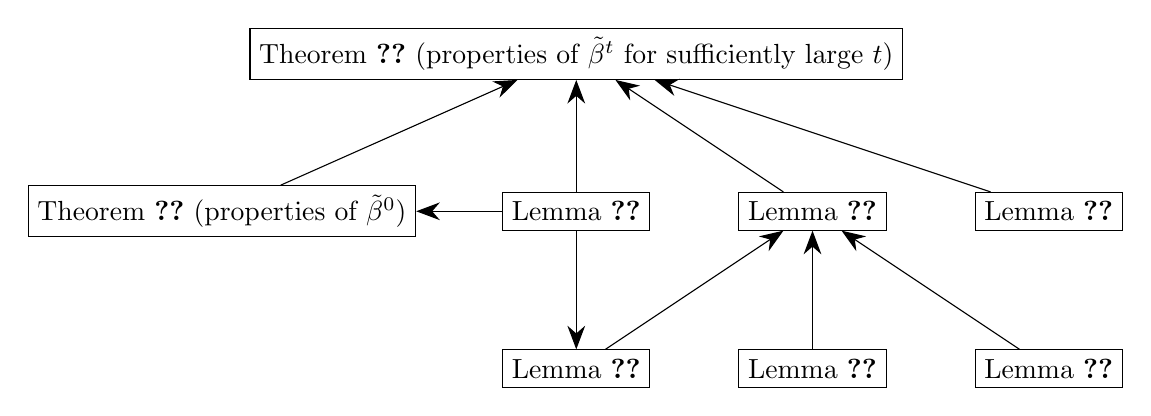
\begin{tikzpicture}[scale = 1]
	\node [draw,rectangle](a)at(-0.5,4){ Theorem \ref{T8} (properties of $\tilde \beta^t$ for sufficiently large $t$)};
	\node [draw,rectangle](b)at(-5,2){ Theorem \ref{upperbound} (properties of $\tilde \beta^0$) };
	\node [draw,rectangle](e)at(-0.5,2){ Lemma \ref{good event} };
	\node [draw,rectangle](f)at(2.5,2){ Lemma \ref{exactOGChi2} };
	\node [draw,rectangle](g)at(5.5,2){ Lemma \ref{exactsupporterror} };
	\node [draw,rectangle](i)at(-0.5,0){ Lemma \ref{exactOGChi2:1st} };
        \node [draw,rectangle](j)at(2.5,0){ Lemma \ref{OGChi2:2nd} };
        \node [draw,rectangle](k)at(5.5,0){ Lemma \ref{OGChi2:3rd} };

	%\draw [->](node cs:name=e,angle=90)|-(n);
        \draw [-{Stealth[length=3mm]}](e)--(a);
        \draw [-{Stealth[length=3mm]}](b)--(a);
        \draw [-{Stealth[length=3mm]}](e)--(b);
        \draw [-{Stealth[length=3mm]}](f)--(a);
        \draw [-{Stealth[length=3mm]}](g)--(a);
        \draw [-{Stealth[length=3mm]}](e)--(i);
        \draw [-{Stealth[length=3mm]}](i)--(f);
        \draw [-{Stealth[length=3mm]}](j)--(f);
        \draw [-{Stealth[length=3mm]}](k)--(f);
\end{tikzpicture}
\caption{A road map to complete the proof of Theorem \ref{T8}. The directed edges mean that the tails of the edges are used in the heads of the edges. }\label{roadmap2}
\end{figure}
 

For $a =1,2$, we define
\begin{equation}\label{mua}
\begin{aligned}
    \mu_a :=& a\sigma \left( \sqrt{ \frac{6}{n} \left( \frac{1}{s_0}\log ({\rm e} m ) +  \log \frac{{\rm e} d}{s_0} \right)  } + \sqrt{ \frac{3}{n} \log(ss_0) } \right)\\
 =&  a\sigma \left( \sqrt{ \frac{6}{n} \Delta(1,s_0) } + \sqrt{ \frac{3}{n} \log(ss_0) } \right),
\end{aligned}
\end{equation}
which leads to $\mu_2 = 2 \mu_1$. This result will be used in \eqref{exactIG}, Lemma \ref{exactOGChi2}, and Lemma \ref{exactOGChi2:1st}.

\begin{proof}[Proof of Theorem \ref{T8}]
First, we show the probability inequalities used in this proof as follows.
\begin{equation}\label{eq:exactprob}
\begin{aligned}
P\left\{ \forall S \in \mathcal S(1,s_0),~\sum_{(i,j) \in S}\tilde \Xi_{ij}^2 
  \le \frac{6\sigma^2 s_0 \Delta(1,s_0)}{n} \right\} &\ge 1- e^{ -\frac18 s_0 \Delta(1,s_0) };\\
P\left\{ \|\tilde\beta^* - \beta^*\|_2^2 = \sum_{(i,j) \in S^*}\left( \tilde\beta_{ij}^* - \beta_{ij}^* \right)^2 \le \frac{6\sigma^2 ss_0}{n(1-\delta)^2} \right\} &\ge 1- \exp\left( -ss_0 \right);\\
P\left\{ \max_{(i,j) \in S^*} |\tilde\beta_{ij}^* - \beta^*_{ij}| 
  \le \sqrt{\frac{3\sigma^2 \log(ss_0)}{n(1-\delta)}}\right\} &\ge 1- 2 (ss_0)^{-1/2}; \\
P\left\{ \max_{(i,j) \in S_{G^*}} |\tilde\Xi_{ij}| 
  \le \sqrt{\frac{3\sigma^2 \log(sd)}{n }}\right\} & \ge 1- 2 (sd)^{-1/2}, \\
\end{aligned}
\end{equation}
where the first and the second inequalities follow from Lemma \ref{good event}, with taking $t=\frac98 s_0 \Delta(1,s_0) $ and $ss_0$ in \eqref{ineq:t} respectively. 
The third and the fourth inequalities follow from the sub-Gaussian property, for example,
\begin{align*}
P\left( \max_{(i,j) \in S_{G^*}} |\tilde\Xi_{ij}| \ge \sqrt{\frac{3\sigma^2 \log(sd)}{n }}\right)
= & P\left( \bigcup_{(i,j) \in S_{G^*}} \left\{ |\tilde\Xi_{ij}| \ge \sqrt{\frac{3\sigma^2 \log(sd)}{n}} \right\}\right)\\
\le & \sum_{(i,j) \in S_{G^*}}2 \exp\left(-\frac{3\log(sd)}{2} \right)\\
\le & \frac{2}{\sqrt{sd}}.
\end{align*}


Now we will prove that the first conclusion in Theorem \ref{T8} holds for all $t \ge 0$. %$\| \tilde \beta^{t} -\tilde \beta^* \|_2 \le 22\left(\frac34 \right)^t \sqrt{ \frac{ \sigma^2 ss_0 \Delta(s,s_0)}{n} } $ holds for all $t \ge 0$.
By Theorem \ref{upperbound}, the initial estimator $\tilde \beta^0$ achieves the minimax estimation rate.
Then, with probability greater than $1-\exp(-ss_0)$, we have 
\begin{equation*}
\begin{aligned}
    \| \tilde \beta^0 -\tilde \beta^* \|_2
\le& \| \tilde \beta^0 - \beta^* \|_2 + \| \beta^*-\tilde \beta^* \|_2\\
\le& \sqrt{ \frac{315\sigma^2 ss_0 \Delta(s,s_0)}{n} } + \sqrt{\frac{6\sigma^2 ss_0}{n(1-\delta)^2} }
< 22\sqrt{ \frac{ \sigma^2 ss_0 \Delta(s,s_0)}{n} } ,
\end{aligned}
\end{equation*}
where the last inequality follows from $\delta < 1/4$. 
By using mathematical induction, we assume that the first conclusion in Theorem \ref{T8} holds for the $t$-th iteration ($t\ge 0$), and we need to prove it still holds for the $(t+1)$-th iteration.

In $(t+1)$-th iteration, we will firstly prove $ \tilde S_{OG}^{t+1} = S_{G^*}^c \cap \tilde S^{t+1} \in \mathcal S(s,s_0) $ and $ \tilde S_{IG}^{t+1} = S_{G^*} \cap (S^*)^c \cap \tilde S^{t+1} \in \mathcal S (s,s_0 ) $ by  contradiction.

\textbf{Step 1 (Control the shape of $ \tilde S_{OG}^{t+1}$ ).} 
By using contradiction, at first, we assume the opposite, that is, $ \tilde S_{OG}^{t+1} $ contains more than $s$ groups (i.e., these groups are not true support groups but the coefficients corresponding to them are not estimated as zero in the $(t+1)$-th iteration). 
Then, we can select arbitrary $s$ falsely discovered groups and construct an index set $S_{OG}' \in \mathcal S (s,s_0)$. The details of the selection process are described as follows:

For any falsely discovered group $G_j$ (i.e., $j \notin G^*$), if $\|\tilde \beta_{G_j}^{t+1}  \|_0 \ge s_0$, then choose arbitrarily $s_0$ non-zero entries from $\tilde \beta_{G_j}^{t+1}$ into $S_{OG}'$;
if $\|\tilde \beta_{G_j}^{t+1}  \|_0 < s_0$, then choose all non-zero entries from $\tilde \beta_{G_j}^{t+1}$ into $S_{OG}'$.
Repeat this operation $s$ times for any $s$ falsely discovered groups, and we obtain a $(s, s_0)$-sparse set $S_{OG}'$, i.e., $S_{OG}' \in \mathcal S(s,s_0)$.

Then, based on the element-wise thresholding operator $\mathcal T_{\mu_2}^{(1)}$ and the group-wise thresholding operator $\mathcal T_{\mu_2,s_0}^{(2)}$, for any group $G_j$ selected by $S_{OG}'$, it holds that 
$$\| \tilde \beta_{G_j \cap S_{OG}'}^{t+1} \|_2^2 
= \left\| \mathcal T_{\lambda_2,s_0}\left(\tilde H^{t+1} \right)_{G_j \cap S_{OG}'} \right\|_2^2 
\ge s_0 \lambda_{2}^2.$$
Based on the decomposition $\tilde H^{t+1}_{ij}
 =  \langle{\Phi}_{(i,j)}^\top,\tilde \beta^*- \tilde \beta^{t}\rangle +  \Xi_{ij}$ (holds for all $ (i,j) \in (S^*)^c$) and triangle inequality, we derive that
\begin{equation}\label{exactOG}
    \begin{aligned}
    \sqrt{ ss_0 }\mu_2
    \le& \sqrt{\sum_{(i,j) \in S_{OG}'} \langle{\Phi}_{(i,j)}^\top, \tilde\beta^* - \tilde\beta^{t} \rangle^2 } 
        + \sqrt{\sum_{(i,j) \in S_{OG}'}  \tilde\Xi_{ij}^2 \mathbf1\Big\{ \mathcal T_{\mu_{2},s_0} 
    \big(\tilde H^{t+1}\big)_{ij}\ne 0\Big\} }\\
    \overset{(i)}{\le} & \delta \|\tilde \beta^t - \tilde\beta^* \|_2 +  \sqrt3 \delta \|\tilde \beta^t - \tilde\beta^* \|_2\\
  \overset{(ii)}{<}& \sqrt{\frac{24\sigma^2 ss_0 \Delta(s,s_0)}{n}}\\
  <& \sqrt{ ss_0 }\mu_2 ,
\end{aligned}
\end{equation}
where inequality (i) follows from \eqref{tech} and Lemma \ref{exactOGChi2}, inequality (ii) follows from the first conclusion in the $t$-th iteration (held by the assumption of induction).
Therefore, we find a contradiction.

Next, we prove that only less than $ss_0$ elements will be falsely discovered outside true groups $G^*$. %(indexed by $\tilde G_{OG}^{t+1}$). 
If not so, we can construct set $S_{OG}'' \in \mathcal S(s,s_0)$, which satisfies that $S_{OG}'' \subseteq \tilde S_{OG}^{t+1}$, $|S_{OG}''|=ss_0$ and each $\tilde \beta_{ij}^{t+1}$ indexed from $S_{OG}''$ is falsely discovered.
Therefore, based on the element-wise thresholding operator and Lemma \ref{exactOGChi2}, we have 
\begin{equation}\label{step1.5}
    \begin{aligned}
    \sqrt{ ss_0 }\lambda_2
    \le& \sqrt{\sum_{(i,j) \in S_{OG}''} \langle{\Phi}_{(i,j)}^\top, \beta^* - \tilde\beta^{t} \rangle^2 } 
        + \sqrt{\sum_{(i,j) \in S_{OG}''} \Xi_{ij}^2 \mathbf1\Big\{ \mathcal T_{\lambda_{2},s_0} 
    \big(\tilde H^{t+1}\big)_{ij}\ne 0\Big\} }\\
    {\le} & (1+\sqrt3)\delta \|\tilde \beta^t - \beta^* \|_2 .
    \end{aligned}
\end{equation}
Then, we similarly find a contradiction as \eqref{exactOG} again.
Therefore, we prove that $S_{G^*}^c \cap \tilde S^{t+1} \in \mathcal S(s,s_0) $.

\textbf{Step 2 (Control the shape of $ \tilde S_{IG}^{t+1} $ ).} 

By using contradiction, at first, we assume the opposite, that is, more than $ss_0$ entries in $S_{G^*}$ are falsely discovered. 
Then we can construct an index set $S_{IG}' \subseteq \tilde S_{IG}^{t+1}$ satisfying $|S_{IG}'| =ss_0$ and $S_{IG}' \in \mathcal S(s,s_0)$, with $|\mathcal T_{\mu_2,s_0} (\tilde H^{t+1})_{ij}| \ge \mu_2$ for all $ (i,j) \in S_{IG}'$. 
Therefore, based on the element-wise thresholding operator, we obtain 
\begin{equation}\label{exactIG}
   \begin{aligned}
    \sqrt{ss_0}\mu_2
    \le & \sqrt{\sum_{(i,j) \in S_{IG}'} \langle{\Phi}_{(i,j)}^\top, \tilde\beta^* - \tilde\beta^{t} \rangle^2 } \\
        &+\sqrt{\sum_{(i,j)\in S_{IG}'}\tilde\Xi_{ij}^2 \mathbf1\Big\{ |\tilde\Xi_{ij}+\langle{\Phi}_{(i,j)}^\top, \tilde\beta^* - \tilde\beta^{t} \rangle|\ge \mu_2 \Big\} }\\
    \le & \delta \|\tilde \beta^t - \tilde\beta^* \|_2
        +\sqrt{\sum_{(i,j)\in S_{IG}'}\tilde\Xi_{ij}^2 \mathbf1\Big\{ |\tilde\Xi_{ij}|\ge \mu_1\Big\} }\\ 
        &+\sqrt{\sum_{(i,j)\in S_{IG}'}\tilde\Xi_{ij}^2 \mathbf1\Big\{ |\tilde\Xi_{ij}|<\mu_1,~|\tilde\Xi_{ij}+ \langle{\Phi}_{(i,j)}^\top, \tilde\beta^* - \tilde\beta^{t} \rangle |\ge \mu_2 \Big\} }\\
    \overset{(i)}{\le}&  \delta \|\tilde \beta^t - \tilde\beta^* \|_2 +\sqrt{\sum_{(i,j)\in S_{IG}'}\tilde\Xi_{ij}^2 \mathbf1\Big\{ |\tilde\Xi_{ij}|<\mu_1 \le |\langle{\Phi}_{(i,j)}^\top, \tilde\beta^* - \tilde\beta^{t} \rangle|\Big\} }\\
    \le & 2 \delta \|\tilde \beta^t - \tilde\beta^* \|_2 ,
\end{aligned}
\end{equation}
where inequality (i) follows from the techniques below: 

By \eqref{mua}, recall that
\begin{align*}
\mu_1
&=  \sqrt{ \frac{6\sigma^2}{n} \left( \frac{1}{s_0}\log({\rm e} m ) + \log\frac{{\rm e} d}{s_0} \right)  }  + \sqrt{ \frac{3\sigma^2}{n} \log(ss_0) } \\ 
&> \sqrt{ \frac{3\sigma^2}{n} \left( \log\frac{{\rm e} d}{s_0} + \log(ss_0) \right)  } \\
&>\sqrt{ \frac{3\sigma^2 \log(sd)}{n}  }.
\end{align*}
Then, by the forth inequality in \eqref{eq:exactprob}, we obtain $ \sum_{(i,j)\in S_{IG}'}\tilde\Xi_{ij}^2 \mathbf1\Big\{ |\tilde\Xi_{ij}|\ge \mu_1\Big\} =0$ with probability greater than $1 - 2(sd)^{-1/2}$. 
Therefore, \eqref{exactIG} leads to a contradiction again as the case in \eqref{exactOG}.


\textbf{Step 3 ($\ell_2$ error inequality of $\tilde \beta^{t+1}$).} 

So far, we have proved that both $ \tilde S_{OG}^{t+1}, \tilde S_{IG}^{t+1} \in \mathcal S(s,s_0) $. 
Note that
\begin{equation}
\begin{aligned}
    &\tilde \beta_{ij}^{t+1} - \tilde \beta_{ij}^* \\
    =& - (\underbrace{\tilde\beta_{ij}^* + \langle{\Phi}_{(i,j)}^\top, \tilde\beta^* - \tilde\beta^{t} \rangle + \tilde\Xi_{ij}}_{\tilde H_{ij}^{t+1}}) \cdot \mathbf1 \left( (i,j) \notin \tilde S^{t+1} \right) + \langle{\Phi}_{(i,j)}^\top, \tilde\beta^* - \tilde\beta^{t} \rangle + \tilde\Xi_{ij},
\end{aligned}
\end{equation}
where recall $ \tilde\Xi_{ij} =0$ for all $ (i,j)\in S^*$, and $ \|\tilde\Xi_{ij}\|_{\psi_2}^2 \le \frac{2\sigma^2}{n}$ for all $ (i,j)\in (S^*)^c$.
We will analyze the estimation error on $S^*$ and $\tilde S^{t+1} \cap (S^*)^c$ respectively. On $S^*$, we have
\begin{equation}\label{eq:exactS*}
\begin{aligned}
\|\tilde \beta_{S^*}^{t+1} - \tilde\beta_{S^*}^* \|_2 
\le& \sqrt{ \sum_{(i,j) \in S^*} \left( \tilde H_{ij}^{t+1} \right)^2 \mathbf1 \left( (i,j) \notin \tilde S^{t+1} \right)}
  + \sqrt{\sum_{(i,j) \in S^*} \langle{\Phi}_{(i,j)}^\top, \tilde\beta^* - \tilde\beta^{t} \rangle^2 }  \\
\overset{(i)}{\le} & \sqrt{ 3+2\sqrt2+\frac1{\epsilon^2} } \delta \left\| \tilde\beta^t - \tilde\beta^* \right\|_2 
  + \delta \left\| \tilde\beta^t - \tilde\beta^* \right\|_2 ,
\end{aligned}
\end{equation}
where inequality (i) follows from Lemma \ref{exactsupporterror} and \eqref{tech}. 

On $\tilde S^{t+1} \cap (S^*)^c$, under DSRIP$(3s,\frac53 s_0, \delta )$ condition, we have 
\begin{equation}\label{eq:exactexceptS*}
\begin{aligned}
& \left\|\tilde \beta_{\tilde S^{t+1} \cap (S^*)^c}^{t+1} \right\|_2\\
\le & \sqrt{\sum_{(i,j) \in \tilde S^{t+1} \cap (S^*)^c} \langle{\Phi}_{(i,j)}^\top, \tilde\beta^* - \tilde\beta^{t} \rangle^2 }\\
& + \sqrt{\sum_{(i,j) \in \tilde S^{t+1} \cap (S^*)^c} \tilde\Xi_{ij}^2 \mathbf1 \left( \mathcal T_{\mu_2,s_0} \big(\tilde H^{t+1}\big)_{ij}\ne 0\right) }\\
\le & \delta \left\| \tilde\beta^t - \tilde \beta^* \right\|_2 \\
& + \sqrt{\sum_{(i,j) \in \tilde S_{OG}^{t+1}} \tilde \Xi_{ij}^2 \mathbf1 \left( \mathcal T_{\mu_2,s_0} \big(\tilde H^{t+1}\big)_{ij}\ne 0\right) 
 +  \sum_{(i,j) \in \tilde S_{IG}^{t+1}} \tilde \Xi_{ij}^2 \mathbf1 \left( \mathcal T_{\mu_2,s_0} \big(\tilde H^{t+1}\big)_{ij}\ne 0\right) }\\
\overset{(i)}{<} & 3 \delta \left\| \tilde\beta^t -\tilde \beta^* \right\|_2,
\end{aligned}
\end{equation}
where inequality (i) is followed by a similar proof as in steps 1 and 2.

Finally, based on \eqref{eq:exactS*}, \eqref{eq:exactexceptS*} and $\delta < \epsilon^4 \wedge \frac2{25} $, we have 
\begin{equation}
    \left\|\tilde \beta^{t+1} - \tilde\beta^* \right\|_2 
    \le  \left\|\tilde \beta_{S^*}^{t+1} - \tilde\beta_{S^*}^* \right\|_2 
         + \left\|\tilde\beta_{\tilde S^{t+1}\cap(S^*)^c}^{t+1}  \right\|_2\\
    %\le & \left( 4+  \sqrt{ 3+2\sqrt2+\frac1{\epsilon^2} } \right) \delta \left\| \tilde\beta^t -\tilde \beta^* \right\|_2\\
    <  \frac35 \left\| \tilde\beta^t -\tilde \beta^* \right\|_2. 
\end{equation}
By initial inequality $\left\| \tilde \beta^0 - \tilde \beta^* \right\|_2 < 22 \sqrt{ \frac{ \sigma^2 ss_0 \Delta(s,s_0)}{n} }$, we conclude that
\begin{equation}
   \left\|\tilde \beta^{t+1} - \tilde \beta^* \right\|_2
<~  22 \left( \frac35 \right)^{t+1}\sqrt{ \frac{ \sigma^2 ss_0 \Delta(s,s_0)}{n} }.
\end{equation}
Therefore, we prove that the first conclusion in Theorem \ref{T8} holds for all $ t \ge 0$.

\textbf{Step 4 (Sharper estimation rate and exact recovery).} 

Next, let $t >  \log \left(  484 n ss_0 \Delta(s,s_0) \right)$, we conclude $ \|\tilde \beta^{t} - \tilde \beta^*  \|_2 < \frac{ \sigma }n$, which leads that 
\begin{equation}\label{eq:8-2}
\left\|\tilde \beta^t -\beta^* \right\|_2
\le \left\|\tilde \beta^t -\tilde \beta^* \right\|_2 + \left\|\tilde \beta^* - \beta^* \right\|_2
\le C\sqrt{\frac{ \sigma^2 ss_0 }{n}},
\end{equation}
and 
\begin{equation}\label{eq:exactfinal}
\left\|\tilde \beta^t -\beta^* \right\|_\infty
\le \left\|\tilde \beta^t -\tilde \beta^* \right\|_\infty + \left\|\tilde \beta^* - \beta^* \right\|_\infty
%\le \left\|\tilde \beta^t -\tilde \beta^* \right\|_2 + 2 \sqrt{\frac{ \sigma^2 \log(ss_0)}n}
< 3 \sqrt{\frac{ \sigma^2 \log(ss_0)}n},
\end{equation}
where the second inequalities in \eqref{eq:8-2} and \eqref{eq:exactfinal} both follow from \eqref{eq:exactprob} and $\delta \le 1/4$.
Then, we conclude that:
\begin{enumerate} 
    \item For every $ (i,j) \in (S^*)^c$, by \eqref{eq:exactfinal}, we have $|\tilde \beta^t_{ij} | <3 \sqrt{\frac{ \sigma^2 \log(ss_0)}{n }} < \mu_2$, which proves that we can not falsely discover any entry by using thresholding parameter $\mu_2$ (just recall the element-wise operator $\mathcal T_{\mu_2}^{(1)} $).

    \item For every $ (i,j) \in S^*$, by \eqref{eq:exactfinal} we obtain that $| \tilde \beta^t_{ij} - \beta_{ij}^*| \le \|\tilde \beta^t -\beta^*  \|_\infty   <3  \sigma \sqrt{ (\log(ss_0))/ n}$.
    Then, by the element-wise beta-min condition we derive that
    \begin{equation*}
        | \beta_{ij}^*| 
        > 2\sqrt{6}\sigma  \sqrt{\frac{\log(ss_0)}n}
        > | \beta_{ij}^* - \tilde \beta^t_{ij} |,
    \end{equation*}
    which proves that the whole support set $S^*$ is recovered with sign consistency.
\end{enumerate}

Therefore, we prove that the second conclusion in Theorem \ref{T8} holds, that is, with probability greater than $1- C_1 \exp(-C_2 s_0 \Delta(1,s_0))-C_3 (ss_0)^{-C_4}$, the true support set $S^*$ can be exactly recovered without any falsely discovered entry for all $ t > \log \left(  484n ss_0 \Delta(s,s_0) \right)$.
\end{proof}

\subsection{Proof of Theorem \ref{T9}}
\begin{proof}[Proof of Theorem \ref{T9}]
By Cram\'er--Wold Theorem, we only need to prove the asymptotic normality for $\sqrt n g^\top (\tilde\beta^t_{S^*} - \beta^*_{S^*})$, where $g \in \mathbb R^{|S^*| \times 1}$ is an arbitrary vector with bounded Euclid norm.
By taking  $t >  \log \left(  484 n ss_0 \Delta(s,s_0) \right)$, the output $\tilde\beta^t$ of Algorithm \ref{scaledIHT} leads that
\begin{align*}
    \left|\sqrt n g^\top (\tilde\beta^t_{S^*} - \beta^*_{S^*}) 
-\sqrt n  g^\top (\tilde\beta^*_{S^*} - \beta^*_{S^*}) \right|
%=\sqrt n \left|g^\top (\tilde\beta^t_{S^*} - \tilde\beta^*_{S^*}) \right|
\le&\sqrt n \|g\|_2 \cdot  \left\| \tilde\beta^t_{S^*} - \tilde\beta^*_{S^*} \right\|_2\\
\le& \|g\|_2 \frac{\sigma}{\sqrt n}
\to 0, 
\end{align*}
as $n,~ p(=d\times m) \to \infty$, where the last inequality follows from Step 4 in the proof of Theorem \ref{T8}.
Therefore we can focus on the term $\sqrt ng^\top (\tilde\beta^*_{S^*} - \beta^*_{S^*})$. By definition we get 
\begin{equation} 
\sqrt n g^\top (\tilde\beta^*_{S^*} - \beta^*_{S^*})
= \sum_{k=1}^n  \sigma\sqrt n \cdot g^\top (X_{S^*}^\top X_{S^*})^{-1} X_{S^*}^{(k)} \xi_k
:= \sum_{k=1}^n \epsilon_k,
\end{equation}
where we denote by $ X_{S^*}^{(k)} \in \mathbb R^{|S^*| \times 1}$ the $k$-th observation of the covariates on the support $S^*$.

Additionally, by DSRIP$(3s,\frac53 s_0, \delta )$ condition we have 
\begin{equation}
    \sum_{k=1}^n\text{Var} \left (  \epsilon_k \right ) 
    = \sigma^2 nc_\xi g^\top (X_{S^*}^\top X_{S^*})^{-1} g
\ge \frac{\sigma^2 c_\xi \|g\|_2^2}{ 1+\delta },
\end{equation}
where recall we define $c_\xi := \text{Var}(\xi_k)$. 
We also have 
\begin{equation}
\begin{aligned}
 \sum_{k=1}^n \mathbf E\left( |\epsilon_k|^3 \right)
=& \sigma^3 n^{3/2}\sum_{k=1}^n \left| g^\top (X_{S^*}^\top X_{S^*})^{-1} X_{S^*}^{(k)}\right|^3 
   \mathbf E\left( |\xi_k|^3 \right)\\
\le& C_1 \sigma^3 n^{3/2} \| g\|_2^3  \left\| (X_{S^*}^\top X_{S^*})^{-1}\right\|_2^3
   \cdot\sum_{k=1}^n\left\|X_{S^*}^{(k)}\right\|_2^3 \\
\le& \frac{C_1 \sigma^3 \| g\|_2^3 }{n^{3/2} (1-\delta)^3} 
   \sum_{k=1}^n \left( ss_0\cdot\max_{(i,j) \in S^*} \left|X_{ij}^{(k)}\right|^2 \right)^{3/2}\\
\le& \frac{C_1 C_2^3 \sigma^3 \| g\|_2^3 (ss_0)^{3/2} }{n^{1/2} (1-\delta)^3} ,
\end{aligned}
\end{equation}
where recall that in Theorem \ref{T9} we assume that $\mathbf E\left( |\xi_k|^3 \right)\le C_1$ and $\left\|X_{S^*} \right\|_{\max} \le C_2$.

Therefore, we have 
\begin{equation}
\begin{aligned}
\frac{1}{\left ( \sum_{k=1}^n\text{Var} \left( \epsilon_k \right) \right )^{3/2} }
\sum_{k=1}^n \mathbf E\left( |\epsilon_k|^3 \right)
\le & \frac{C_1 C_2^3 \sigma^3 \| g\|_2^3 (ss_0)^{3/2} (1+\delta)^{3/2}}
{n^{1/2} (1-\delta)^3 \sigma^3 c_\xi^{3/2} \|g\|_2^3  }\\
=& \frac{C_1 C_2^3   (1+\delta)^{3/2} }
{c_\xi^{3/2} (1-\delta)^3 } \cdot \sqrt{\frac{(ss_0)^3}{n}} 
\to 0,
\end{aligned}
\end{equation}
as $ss_0 = o(n^{1/3})$ and $n\to \infty$.
Finally, by Lyapunov central limit theorem, we conclude that 
$$
\frac{\sqrt n g^\top (\tilde\beta^*_{S^*} - \beta^*_{S^*})}
{\sqrt{\sigma^2 c_\xi g^\top \left( \frac1n X_{S^*}^\top X_{S^*} \right)^{-1} g }} \to N(0,1),
$$
as $n, p \to \infty$ and $ss_0 = o(n^{1/3})$, and hence we complete the proof of Theorem \ref{T9}. 
\end{proof}

\section{Proof of the minimax lower bounds}\label{lowerproof}
First, we consider the minimax lower bound for signal estimation and transform the minimax risk into Bayesian risk for in-depth analysis. This analytical framework is inspired by \cite{MN19}.

\begin{lemma}\label{lemma:minimaxori}
For any $1\le s<m,~1\le s_0<d$, any subset ${\Theta} \subseteq \mathbb R^p$ and for any prior probability distribution $\pi$ on $\mathbb R^p$, as we assume the design matrix $X \in \mathbb R^{n \times p}$ is fixed, we have
\begin{equation}\label{lemma1.ineq}
\begin{aligned} 
&\inf_{\hat \beta} \sup_{\beta^* \in {\Theta}} \underset{Y \sim P_{\beta^*}}{\mathbf{E}}\|\hat \beta - \beta^* \|_2^2 \\
\ge & \inf_{\hat T  } \underset{\beta^* \sim \pi}{\mathbf{E}}~ 
      \underset{Y \sim P_{\beta^*}}{\mathbf{E}} \|\hat T(Y,X) - \beta^* \|_2^2\\
& - 2\underset{\beta^* \sim \pi}{\mathbf {E}}~ \underset{Y \sim P_{\beta^*}}{\mathbf{E}}
      \Bigg\{\bigg(\underset{\beta^{ {\Theta}} | Y}{\mathbf{E} }\Big(\left\|\beta^{ {\Theta}}\right\|_2^2 \big| Y\Big)+\|\beta^*\|_2^2\bigg) \mathbf{1}\left(\beta^* \notin {\Theta} \right)\Bigg\},
\end{aligned}
\end{equation}
where $\inf_{\hat \beta}, \inf_{\hat T  }$ are taken over all estimator of $\beta^*$, $\beta^{ {\Theta}}:= \beta \mathbf1(\beta \in {\Theta})$, and We assume the prior distribution of $\beta $ is independently identical with the prior of $\beta^{*}$. 
Denote by $\underset{\beta^{ {\Theta}} | Y}{\mathbf{E} }(\cdot|Y)$ an expectation based on the conditional distribution $\frac{ P(Y|\beta) \mathrm d \pi_{\Theta}(\beta) }{ \int  P(Y|\beta ) \mathrm d \pi_{\Theta}(\beta ) }$, where $\pi_{\Theta}$ denotes the probability measure $\pi$ conditioned by the event $\{ \beta \in {\Theta} \}$.
\end{lemma}


\subsection{Lower bounds based on Bernoulli prior}\label{Bernoulli}
Recall that we mainly focus on two subsets of ${\Theta}(s,s_0,a)$, which can be described as 
\begin{align*}
{\Theta}_1 &: = \Big\{\beta \in {\Theta}(s,s_0,a): 
~ G^*(\beta ) = [s]; ~ \| \beta\|_0 = ss_0;\\
&\qquad\qquad\qquad\qquad\qquad \beta_{ij} = a \text{  for all } (i,j) \in S^*(\beta) \Big\},\\
{\Theta}_2&: = \Big\{{\beta} \in {\Theta}(s,s_0,a): 
~ |G^*(\beta)| = s;~ \beta_{ij} =a  \text{  for all }  i \in [s_0], j \in G^*(\beta) \Big\}.
\end{align*}
In ${\Theta}_1$, information is limited to the location of support groups, omitting details on their support entries. 
While ${\Theta}_2$ provides insight into the support entries within support groups, it lacks information on the location of support groups.
Given the aforementioned settings, we frame the signal estimation as a support identification problem,
i.e., to estimate the decoder $\eta^* = \{\mathbf{1}(\beta^*_{ij} \ne 0) \}_{ij}\in \{0,1\}^{p}$. 
Recall that we assume that $X$ satisfies DSRIP$(s,s_0,\delta)$ condition with some constant $\delta \in (0,1)$. This assumption will be used in the proof of Theorem \ref{allselectorD1D2} and \ref{LB2priors}.
Plus, we define two useful functions:
\begin{equation}\label{aux2fun}
\begin{aligned}
    \psi(d,s_0,a,\sigma) &:=(d-s_0){\Phi}\left(-\frac{t(a,d,s_0,\sigma)}{\sigma}\right) + s_0 {\Phi}\left(-\frac{a\sqrt n-t(a,d,s_0,\sigma)}{\sigma}\right),\\
    t(a,d,s_0,\sigma) &:= \frac{a\sqrt n}{2} + \frac{\sigma^2}{a\sqrt n} \log \frac{d-s_0}{s_0}.
\end{aligned}
\end{equation}
 
\subsection*{B.2 Proof of Theorem \ref{allselectorD1D2}}
%We use two Bernoulli prior distributions to lower bound the losses on ${\Theta}_1$ and ${\Theta}_2$ respectively. 
%Specifically, based on $\eta \to \beta \to Y$ and $Y \sim P_{\beta}$ for the fixed matrix $X$,
%({here we assume each $\eta \in \{0,1\}^{p}$ corresponds only one $\beta \in \mathbb R^{p}$ and one distribution of Y, as $P_\eta$})
%we can get estimator $\hat \eta = \hat \eta(Y,X) \in \mathbb R^{p}$, and call $\hat \eta_{ij}$ is the estimator (or selector) of $\eta_{ij} = \mathbf1(\beta_{ij} \ne 0)$, i.e., the sign of whether the $i$-th variable in the $j$-th group is in the support set.
 
Now, we define two prior distributions $\pi_1$ and $\pi_2$ corresponding to parameter subsets ${\Theta}_1$ and ${\Theta}_2$ respectively.
For $\pi_1$, suppose that for each $(i,j) \in [d] \times [s]$ (note by the definition of ${\Theta}_1$, the support index must be in $[d] \times [s]$), the number of support entries is from a binomial distribution, that is, $\sum_{(i,j) \in [d] \times [s]} \eta_{ij}^* \sim Bin (ds, s_0'/d)$, where $ s_0' $ satisfies $1\le s_0' < s_0$ is an integer determined later. 
And assume that $\eta_{G_j}^* \equiv \mathbf 0_d$ for all $ j >s$.

For $\pi_2$, suppose that the number of support groups is from a binomial distribution $Bin(m, s^{\prime} / m)$, where $ s' < s$ is also an integer determined later.
In each support group, only the first $s_0$ entries are support entries. Therefore $\eta_{ij}^* \equiv 0$ for all $i > s_0, j \in [m]$.

Note that $\pi_1$ and $\pi_2$ are two prior distributions of $\eta^*$, while $\beta^* = a\cdot\eta^*$ in ${\Theta}_1$ and ${\Theta}_2$.
%By letting $\beta = a \eta_k$, we can also get the prior distributions of $\beta$ for $k=1,2$ respectively. 
Therefore, $a \hat \eta$ can also be an efficient estimator of $\beta^*$ for those $\beta^* \in {\Theta}_1 \cup {\Theta}_2$.
Therefore, we replace $\beta^*$ and $\hat \beta$ (in Lemma \ref{lemma:minimaxori}) by $\eta^*$ and $\hat \eta$ with prior $\pi_k$ (for $k=1,2$), and directly have
\begin{equation}\label{eq:priork}
\begin{aligned}
&\inf_{\hat \eta} \sup_{\beta^* \in  {\Theta}_k} 
    \mathbf{E}_{Y\sim P_{\beta^*} } \|\hat \eta - \eta^*\|_2^2 \\
\ge &\inf_{\hat T } \underset{\eta^* \sim \pi_k}{\mathbf E} \underset{Y \sim P_{\beta^*} }{\mathbf E} \|\hat T(Y,X) - \eta^*\|_2^2 \\
    &-2 \underset{\eta^* \sim \pi_k}{\mathbf E} \underset{Y \sim P_{\beta^*} }{\mathbf E}  \Bigg\{ \bigg( \underset{\eta^{ {\Theta}_k}|Y}{\mathbf{E}}   \Big( \|\eta^{ {\Theta}_k} \|_2^2 \big| Y \Big) +
    \| \eta^* \|_2^2  \bigg) \mathbf1( a\eta^* \notin {\Theta}_k) \Bigg\} \\
\ge &\inf_{\hat T } \underset{\eta^* \sim \pi_k}{\mathbf E} \underset{Y \sim P_{\beta^*} }{\mathbf E}  \|\hat T(Y,X) - \eta^* \|_2^2 \\
    &-2 ss_0 \underset{\eta^* \sim \pi_k}{\mathbf E} \big( \mathbf1( a\eta^* \notin {\Theta}_k) \big) 
    -2 \underset{\eta^* \sim \pi_k}{\mathbf E} \big( \| \eta^*\|_2^2 \mathbf1( a\eta^* \notin {\Theta}_k) \big),
\end{aligned}
\end{equation}
where $\inf_{\hat T}$ denotes the infimum over all estimators $\hat T \in [0,1]^p$, and the last inequality follows from $\|\eta^{ {\Theta}_k} \|_2^2 =  \|\eta \|_2^2\cdot \mathbf1( a\eta \in  {\Theta}_k )\le ss_0$.

\begin{proof}[Proof of \eqref{allselectorD1}]

Recall that by $\beta^* \in {\Theta}_1$, only the first $s$ groups are support groups.
And based on the prior $\pi_1$, the total number of support entries is from a binomial distribution $Bin(ds, s_0' / d)$ independently, where $ s_0' < s_0$. 
\begin{comment}
Based on $\beta_{ij}^* =a\cdot\eta_{ij}^* $, from \eqref{eq:priork} we have
\begin{equation}\label{eq:priork}
\begin{aligned}
& \inf_{\hat \eta} \sup_{\beta^* \in {\Theta}_1} \mathbf{E}_{Y\sim P_{\beta^*} } \| \hat \eta - \eta^* \|_2^2 \\
\ge& \inf_{\hat T } 
     \mathbf E_{\eta^* \sim \pi_1} \mathbf E_{Y \sim P_{\beta^*} } \|\hat T(Y,X) - \eta^* \|_2^2
    - 2ss_0 \mathbf E_{\eta^* \sim \pi_1} \Big( \mathbf1( a\eta^* \notin {\Theta}_1)  \Big)
    - 2 \mathbf E_{\eta^* \sim \pi_1}  \Big( \|\eta^* \|_2^2 \mathbf1( a\eta^* \notin {\Theta}_1) \Big).
\end{aligned}
\end{equation}
\end{comment}
Under prior $\pi_1$, for the last two terms in \eqref{eq:priork}, let $v:= \sum_{(i,j)\in [d]\times [s]} \eta_{ij}^* {\sim} Bin(ds , s_0'/d)$, therefore we have 
\begin{equation}\label{eq:23term}
   \begin{aligned}
&2ss_0 \mathbf E_{\eta^* \sim \pi_1} \Big( \mathbf1( a\eta^* \notin {\Theta}_1)  \Big) + 2\mathbf E_{\eta^* \sim \pi_1}  \Big( \|\eta^*\|_2^2 \mathbf1(a\eta^* \notin {\Theta}_1) \Big)\\
\le& 2ss_0 \mathbf P \left( v > ss_0\right)
    + 2\mathbf E \left( v\mathbf1(v  >ss_0)  \right)\\
\le& 2s s_0 \exp\left(-\frac{s(s_0-s_0')^2}{2s_0}\right) 
    +ss_0' \exp\left(-\frac{s(s_0-s_0')^2}{2s_0}\right)\\
\le & (2s s_0+ ss_0') \exp\left(-\frac{s(s_0-s_0')^2}{2s_0}\right) ,
\end{aligned}
\end{equation}
where the first and the final inequalities follow from Lemma \ref{berncen}, and the final inequality also follows from 
\begin{equation*}
\begin{aligned}
&\mathbf E\left(  v \mathbf1(v > ss_0) \right)\\
=&\sum_{i=ss_0+1}^{ds} i \binom{ds}{i} \left( \frac{ss_0' }{ds} \right)^i \left(1- \frac{ss_0'}{ds} \right)^{ds-i}\\
=& ss_0' \sum_{i-1=ss_0}^{ds-1} \frac{(ds-1)!}{(i-1)!~[(ds-1)-(i-1)]!} \left( \frac{ss_0'}{ds} \right)^{i-1} \left(1- \frac{ss_0'}{ds} \right)^{(ds-1)-(i-1)}\\
=& ss_0' P\left( Bin(ds-1 , \frac{s_0'}{d} ) \ge ss_0\right)
\le s s_0' P\left( Bin(ds , \frac{s_0'}{d} ) \ge s s_0\right)\\
\le& ss_0' \exp\left(-\frac{s(s_0-s_0')^2}{2s_0}\right). 
\end{aligned}
\end{equation*}
 
For the first term in \eqref{eq:priork}, define
\begin{equation*}
\tilde Y_{ij}:= Y - \sum_{(k,\ell) \ne (i,j)} X_{(k\ell)} ~ \beta_{k\ell}^* = X_{(ij)} \beta_{ij}^* + \sigma \xi.
\end{equation*}
Then we have
\begin{align*}
& \inf_{\hat T }\underset{\eta^* \sim \pi_1}{\mathbf E}
    \underset{Y \sim P_{\beta^*} }{\mathbf E} \|\hat T(Y,X) - \eta^* \|_2^2 \\
\overset{(i)}{\ge} & \sum_{j=1}^s \sum_{i=1}^d \underset{\eta_{\setminus (ij)}^* }{\mathbf E}
    \left\{ \inf_{\hat T_{ij} }
    \underset{\eta_{ij}^* }{\mathbf E} \underset{Y}{\mathbf E}
    \left( (\hat T_{ij}(Y,X) - \eta_{ij}^*)^2 \Big| \eta_{\setminus (ij)}^* \right) \right\} \\
\overset{(ii)}{=}& \sum_{j=1}^s \sum_{i=1}^d \underset{\eta_{\setminus (ij)}^* }{\mathbf E} \left\{ \inf_{\hat T_{ij} }
    \underset{\eta_{ij}}{\mathbf E} \underset{Y}{\mathbf E}
    \left( (\hat T_{ij}(\tilde Y_{ij},X) - \eta_{ij}^*)^2 \Big| \eta_{\setminus (ij)}^* \right) \right\} \\
%= &  \sum_{j=1}^s \sum_{i=1}^d \underset{\eta_{\setminus (ij)}}{\mathbf E}  \left\{ \inf_{\hat T_{ij} } \underset{\eta_{ij}}{\mathbf E} \left( \mathbf1(\eta_{ij}=0)
%    \underset{\tilde Y_{ij}|\eta_{ij}=0}{\mathbf E} |\hat T_{ij}(\tilde Y_{ij},X)|^2  
%    + \mathbf1(\eta_{ij}=1) \underset{\tilde Y_{ij}|\eta_{ij}=1}{\mathbf E}  |1-\hat T_{ij}(\tilde Y_{ij},X)|^2  \right) \right\}\\
=& \sum_{j=1}^s \sum_{i=1}^d  \inf_{\hat T_{ij}} \left\{
    \left(1-\frac{s_0'}{d}\right)
    \underset{\tilde Y_{ij}\sim N(\mathbf 0,\sigma^2 \mathbf I_n)}{\mathbf E}
     \left( \hat T_{ij}(\tilde Y_{ij},X) \right)^2\right. \\
    &  \qquad\qquad \qquad \left.+ \frac{s_0'}{d} \left(
    \underset{\tilde Y_{ij} \sim  N(aX_{ij},\sigma^2 \mathbf I_n)}{\mathbf E} \left( 1 -\hat T_{ij}(\tilde Y_{ij},X) \right)^2
    \right) \right\}.
\end{align*}
where inequality (i) only considers the first $s$ groups since we can always set $\hat T_{ij} = 0$ for all $ j>s, i \in [d]$ because of the structure of $\pi_1$.
Equality (ii) is based on that under independent prior distributions of the entries of $\eta^*$, the oracle selector of a given component $\eta_{ij}^*$ does not depend on the rest of the components. 
And %by the Bayesian version of the Neyman-Pearson lemma, 
the infimum in the last equality can be achieved by the selector 
\begin{equation*}
\hat T_{ij}^{*}(\tilde Y_{ij},X) 
:= \frac{1}{1+ \frac{(d-s_0')\boldsymbol \varphi_{\sigma} ( \tilde Y_{ij})  }
    {s_0' \boldsymbol \varphi_{\sigma} (\tilde Y_{ij}-aX_{ij} ) } }
=\frac{1}{1+ \frac{d-s_0'}{s_0'}
   \frac{\boldsymbol \varphi_{0,\sigma}(\tilde Y_{ij})}{\boldsymbol \varphi_{a,\sigma}(\tilde Y_{ij}) } },
\end{equation*}
where we abbreviate $\boldsymbol \varphi_{0,\sigma}({\tilde Y_{ij}}):= \boldsymbol \varphi_{\sigma} ( \tilde Y_{ij})$, $\boldsymbol \varphi_{a,\sigma} (\tilde Y_{ij} ):= \boldsymbol \varphi_{\sigma} (\tilde Y_{ij}-aX_{ij} )$, and $\boldsymbol \varphi_{ \sigma}(y) = \frac{1}{\sqrt{2\pi}\sigma} \exp \left( - \frac{y^2}{2\sigma^2} \right)$.
Then, define event $\mathcal A := \left\{\mathbf y \in R^n : ~\frac{d-s_0'}{s_0'} \frac{\boldsymbol \varphi_{0,\sigma}(\mathbf y)}{\boldsymbol \varphi_{a,\sigma}(\mathbf y) } >1 \right\}$, after some simple calculation we have 
\begin{equation}\label{D1T}
\begin{aligned}
&\inf_{\hat T\in[0,1]^p}\underset{\eta^* \sim \pi_1}{\mathbf E} 
   \underset{Y \sim P_{\beta^*} }{\mathbf E} \|\hat T(Y,X) - \eta^* \|_2^2 \\
%\ge& sd \left\{ \int_{{\bf y} \in \mathbb R^n} \frac{d-s_0'}{d} \left( \frac{1}{1+ \frac{d-s_0'}{s_0'}
 %  \frac{\boldsymbol \varphi_{0,\sigma}({\bf y})}{\boldsymbol \varphi_{a,\sigma}({\bf y})}}
%   \right)^2 \boldsymbol \varphi_{0,\sigma}({\bf y})
%   + \frac{s_0'}{d}\left( \frac{\frac{d-s_0'}{s_0'} \frac{\boldsymbol\varphi_{0,\sigma}({\bf y})}{\boldsymbol \varphi_{a,\sigma}({\bf y})}}
%   {1+\frac{d-s_0'}{s_0'} \frac{ \boldsymbol \varphi_{0,\sigma}({\bf y})}{\boldsymbol \varphi_{a,\sigma}({\bf y})}}\right)^2
%   \boldsymbol \varphi_{a,\sigma}({\bf y}) \mathrm d {\bf y} \right\} \\
\ge& sd\int_{{\bf y}\in \mathcal A} \frac{s_0'}{d} \frac{\frac{d-s_0'}{s_0'} \frac{\boldsymbol\varphi_{0,\sigma}({\bf y})}{\boldsymbol \varphi_{a,\sigma}({\bf y})}}
   {1+\frac{d-s_0'}{s_0'} \frac{ \boldsymbol \varphi_{0,\sigma}({\bf y})}{\boldsymbol \varphi_{a,\sigma}({\bf y})}}
   \boldsymbol \varphi_{a,\sigma}({\bf y}) \mathrm d {\bf y}
    + sd\int_{{\bf y}\in \mathcal A^c} \frac{s_0'}d \frac{\frac{d-s_0'}{s_0'} \frac{\boldsymbol\varphi_{0,\sigma}({\bf y})}{\boldsymbol \varphi_{a,\sigma}({\bf y})}}
   {1+\frac{d-s_0'}{s_0'} \frac{ \boldsymbol\varphi_{0,\sigma}({\bf y})}{\boldsymbol \varphi_{a,\sigma}({\bf y})}}
   \boldsymbol \varphi_{a,\sigma}({\bf y}) \mathrm d {\bf y}\\
\ge&sd \int_{{\bf y}\in \mathcal A} \frac{s_0'}{d} \cdot \frac12 \boldsymbol \varphi_{a,\sigma}({\bf y})\mathrm d {\bf y}
    +sd \int_{{\bf y}\in \mathcal A^c} \frac{d-s_0'}{d} \cdot\frac12 \boldsymbol \varphi_{0,\sigma}({\bf y})\mathrm d {\bf y}\\
=& \frac{sd}{2} \left\{ \frac{s_0'}{d} {\Phi}\left(-\frac{a \sqrt n}{2\sigma}+\frac{\sigma}{a\sqrt n} \log\frac{d-s_0'}{s_0'}\right) \right.\\
  &\qquad \left.  + \frac{d-s_0'}{d} {\Phi}\left(-\frac{a \sqrt n}{2\sigma}-\frac{\sigma}{a\sqrt n} \log\frac{d-s_0'}{s_0'}\right) \right\}\\
=& \frac{s}{2} \psi(d, s_0', a, \sigma)
\end{aligned}
\end{equation}

Combining \eqref{eq:priork}, \eqref{eq:23term} and \eqref{D1T} together, we have
\begin{equation}\label{Theta1}
\begin{aligned}
& \inf_{\hat \eta} \sup_{\beta \in {\Theta}_1} \mathbf{E}_{Y\sim P_\beta} \| \hat \eta(Y,X) - \eta \|_2^2 \\
%\ge& \inf_{\hat T\in[0,1]^p} \underset{\beta \sim \pi_1}{\mathbf E} \underset{Y \sim P_\beta}{\mathbf E} \|\hat T(Y,X) - \eta\|_2^2 
%    -2 ss_0 \underset{\beta \sim \pi_1}{\mathbf E} \big[ \mathbf1(\beta \notin {\Theta}_1) \big]  -2 \underset{\beta \sim \pi_1}{\mathbf E} \big[ \|\eta\|_1 \mathbf1(\beta \notin {\Theta}_1) \big]\\
%\ge& \frac{sd}{2} \left\{ \frac{d-s_0'}{d} {\Phi}\left(-\frac{a \sqrt n}{2\sigma}-\frac{\sigma}{a\sqrt n} \log\frac{d-s_0'}{s_0'}\right) 
%    + \frac{s_0'}{d} {\Phi}\left(-\frac{a \sqrt n}{2\sigma}+\frac{\sigma}{a\sqrt n} \log\frac{d-s_0'}{s_0'}\right) \right\} \\
%    &-(2s s_0+ ss_0') \exp\left(-\frac{s(s_0-s_0')^2}{2s_0}\right) \\
\ge& \frac{s}{2} \psi(d, s_0', a, \sigma) 
    -(2s s_0+ ss_0') \exp\left(-\frac{s(s_0-s_0')^2}{2s_0}\right)\\
{\ge}& \frac{ss_0'}{2s_0}\psi(d, s_0, a, \sigma) 
    -(2s s_0+ ss_0') \exp\left(-\frac{s(s_0-s_0')^2}{2s_0}\right), \\
\end{aligned}
\end{equation}
where the last inequality follows from Lemma \ref{mdPsi}.
\end{proof}

\begin{proof}[Proof of \eqref{allselectorD2}]
Let $u$ denote the number of support groups in $\beta^*$.
By the prior $\pi_2$, we have $u \sim Bin(m, s^{\prime} / m)$, where $ s^{\prime} < s$. 
By $\beta^* \in {\Theta}_2$, for each support group, only the first $s_0$ entries are support entries. 
\begin{comment}
Then, by $\beta^* = a \cdot \eta^*$, from \eqref{eq:priork} we have
\begin{equation}\label{eq:priork}
\begin{aligned}
&\inf_{\hat \eta} \sup_{\beta^* \in  {\Theta}_2} 
    \mathbf{E}_{Y\sim P_{\beta^*} } \|\hat \eta - \eta^* \|_2^2 \\
\ge &\inf_{\hat T } \underset{\eta^* \sim \pi_2}{\mathbf E} \underset{Y \sim P_{\beta^*} }{\mathbf E} \|\hat T(Y,X) - \eta^* \|_2^2 
    -2 ss_0 \underset{\eta^* \sim \pi_2}{\mathbf E} \big( \mathbf1(a\eta^* \notin {\Theta}_2) \big)
    -2 \underset{\eta^* \sim \pi_2}{\mathbf E} \big( \|\eta\|_2^2 \mathbf1( a\eta^*  \notin {\Theta}_2) \big).
\end{aligned}
\end{equation}
\end{comment}
Under prior $\pi_2$, for the last two terms of \eqref{eq:priork}, similarly as \eqref{eq:23term}, we have 
\begin{equation}
 \begin{aligned}
&2 ss_0 \underset{\eta^* \sim \pi_2}{\mathbf E} \big( \mathbf1(a\eta^* \notin {\Theta}_2) \big) + 2 \underset{\eta^* \sim \pi_2}{\mathbf E} \big( \|\eta\|_2^2 \mathbf1( a\eta^* \notin {\Theta}_2) \big)\\
=& 2ss_0 \mathbf P_{u} \Big( u > s\Big)
    + 2s_0 \mathbf E_{u} \Big( u\mathbf1(u>s) \Big)\\
\le& (2ss_0+2s_0s^\prime)\exp\left(-\frac{(s-s^\prime)^2}{2s} \right).
\end{aligned}
\end{equation}

For the first term of \eqref{eq:priork}, we have
\begin{align*}
& \inf_{\hat T }\underset{\eta^* \sim \pi_2}{\mathbf E}~
    \underset{Y \sim P_{\beta^*} }{\mathbf E} \|\hat T(Y,X) - \eta^* \|_2^2\\
\overset{(i)}=&\inf_{\hat T } \sum_{j=1}^m \underset{\eta_{\setminus G_j}^*}{\mathbf E}  \left\{
    \underset{\eta_{G_j}^*}{\mathbf E}\underset{Y }{\mathbf E} \left( \sum_{i=1}^{s_0} |\hat T_{ij}(Y,X) - \eta_{ij}^*|^2 \Big| \eta_{\setminus G_j}^* \right) \right\}\\ 
\ge &\sum_{j=1}^m \underset{\eta_{\setminus G_j}^* }{\mathbf E}  \left\{ \inf_{\hat T_{G_j} }~
    \underset{\eta_{G_j}^* }{\mathbf E}\underset{Y }{\mathbf E} \left( \sum_{i=1}^{s_0} |\hat T_{ij}(Y,X) - \eta_{ij}^*|^2 \Big| \eta_{\setminus G_j}^* \right) \right\}\\ 
\overset{(ii)}{\ge}& \sum_{j=1}^m \underset{\eta_{\setminus G_j }^*}{\mathbf E}
    \left\{ \inf_{\hat T_{G_j}}~ \underset{\eta_{G_j}^* }{\mathbf E} 
    \left( \mathbf1(\eta_{G_j}^* =\mathbf0_d )~ \underset{\tilde Y_{G_j}|\eta_{G_j}^* =\mathbf0_d}{\mathbf E}
    \left[ \sum_{i=1}^{s_0} (\hat T_{ij}(\tilde Y_{G_j} , X))^2
    \Big | \eta_{\setminus G_j}^* \right] \right.\right.\\
    &\qquad\qquad\qquad + \left.\left. \mathbf1(\eta_{G_j}^* \ne \mathbf 0_d)~ \underset{\tilde Y_{G_j}|\eta_{G_j}^* \ne \mathbf0_d}{\mathbf E}
    \left[\sum_{i=1}^{s_0}\big(1-\hat T_{ij}(\tilde Y_{G_j} ,X)\big)^2
    \Big| \eta_{\setminus G_j}^* \right] \right) \right\} \\ 
\ge & \sum_{j=1}^m \underset{\eta_{\setminus G_j}^* }{\mathbf E}  
    \left\{ \inf_{\hat T_{G_j}} \left( \frac{m-s'}{m}~
    \underset{ \tilde Y_{G_j} |\eta_{G_j}^* =\mathbf0_d}{\mathbf E} \left[ 
    \frac{1}{s_0} \left(\sum_{i=1}^{s_0} \hat T_{ij}(\tilde Y_{G_j},X)\right)^2 
    \Big|\eta_{\setminus G_j}^* \right] \right.\right.\\
    &\qquad\qquad\qquad \left.\left.+ \frac{s'}{m}~\underset{\tilde Y_{G_j} |\eta_{G_j}^* \ne \mathbf0_d}{\mathbf E}
    \left[  \frac{1}{s_0} \left( s_0 -\sum_{i=1}^{s_0} \hat T_{ij}(\tilde Y_{G_j},X) \right)^2  \Big| \eta_{\setminus G_j}^* \right]  \right) \right\}\\ 
\overset{(iii)}{\ge} & \frac{1}{s_0} \sum_{j=1}^m \underset{\eta_{\setminus G_j}^* }{\mathbf E}  
    \left\{ \inf_{\widehat{ST}_{j}} \left[ \frac{m-s'}{m}
    \underset{\tilde Y_{G_j}|\eta_{G_j}^* =\mathbf0_d}{\mathbf E} \left(
    \widehat{ST}_{j}^2 \Big| \eta_{\setminus G_j}^*  \right)  \right.\right. \\
    & \qquad\qquad\qquad\qquad \left.\left.+ \frac{s^\prime}{m}~\underset{\tilde Y_{G_j}|\eta_{G_j}^* \ne \mathbf0_d}{\mathbf E}
    \left( (s_0-\widehat{ST}_{j} )^2 \Big| \eta_{\setminus G_j}^*  \right) \right] \right\},
\end{align*}
where inequality (i) only considers the first $s_0$ entries in each group. 
This is because, according to the definition of prior $\pi_2$, $\eta_{ij}^* \equiv 0$ for all $ i>s_0$ and $j \in [m]$, therefore we can always set $\hat T_{ij} = 0$ for all $ i>s_0$ and $j \in [m]$.
In inequality (ii), we use
\begin{equation*}
\tilde Y_{G_j}:= Y - \sum_{k \ne j}\sum_{i \in[s_0]} \beta_{ik}^* X_{(ik)} = \sum_{i\in[s_0]} a \eta_{ij}^* X_{(ij)} + \sigma \xi \in \mathbb R^n
\end{equation*}
to represent the marginal observation under the information of the other groups.
Again, the infimum of inequality (iii) can be achieved by the selector
\begin{equation} 
\widehat{ST}_{j}^{*}(\tilde Y_{G_j},X) 
:=  \frac{s_0}{ 1+ \frac{m-s'}{s'} \frac {\boldsymbol \varphi_{\sigma}(\tilde Y_{G_j})}
    {\boldsymbol \varphi_{\sigma} \left( \tilde Y_{G_j}-\sum_{i\in [s_0]}a X_{(ij)}\right)} }.
\end{equation}

Recall that the support variables are orthogonal in each support group.
Therefore, leveraging a technique similar to \eqref{D1T}, we obtain
\begin{equation}\label{D2T}
\begin{aligned}
&\inf_{\hat T }\underset{\eta \sim \pi_2}{\mathbf E} ~
   \underset{Y \sim P_\beta}{\mathbf E} \|\hat T(Y,X) - \eta\|_2^2 \\
\ge& \frac{s_0}{2m}\sum_{j=1}^m \left\{ (m-s'){\Phi}\left(-\frac{a \|\sum_{i\in[s_0]}X_{(ij)}\|_2}{2\sigma}-\frac{\sigma \log(m/s'-1)}{a\|\sum_{i\in[s_0]}X_{(ij)}\|_2 } \right)  \right.\\
  & \quad\quad\quad\quad \left.+ s'{\Phi}\left(-\frac{a \|\sum_{i\in[s_0]}X_{(ij)}\|_2 }{2\sigma} + \frac{\sigma \log(m/s'-1)}{a \|\sum_{i\in[s_0]}X_{(ij)}\|_2 } \right) \right\}\\ 
\overset{(i)}{\ge}& \frac{s_0 s'}{2m s}\sum_{j=1}^m \left\{ (m-s){\Phi}\left(-\frac{a \|\sum_{i\in[s_0]}X_{(ij)}\|_2}{2\sigma}-\frac{\sigma \log(m/s-1)}{a\|\sum_{i\in[s_0]}X_{(ij)}\|_2 } \right)  \right.\\
  & \quad\quad\quad\qquad \left.+ s{\Phi}\left(-\frac{a \|\sum_{i\in[s_0]}X_{(ij)}\|_2 }{2\sigma} + \frac{\sigma \log(m/s-1)}{a \|\sum_{i\in[s_0]}X_{(ij)}\|_2 } \right) \right\}\\ 
\overset{(ii)}{\ge}& \frac{ s_0 s'}{2s} \left\{ (m-s) {\Phi}\left(-\frac{a \sqrt{n(1+\delta)s_0}}{2\sigma}-\frac{\sigma \log(m/s-1)}{a\sqrt{n(1-\delta)s_0}} \right) \right.\\
& \qquad\quad \left.+  s {\Phi}\left(-\frac{a \sqrt{(1+\delta)ns_0}}{2\sigma}+\frac{\sigma \log(m/s-1) }{a\sqrt{(1+\delta)ns_0}}\right) \right\} ,
\end{aligned}
\end{equation}
where inequality (i) follows Lemma \ref{mdPsi}, inequality (ii) follows DSRIP condition.

Combining \eqref{eq:priork}-\eqref{D2T} together, we have
\begin{equation}
\begin{aligned}
& \inf_{\hat \eta} \sup_{\beta \in {\Theta}_2} \mathbf{E}_{Y\sim P_\beta} \|\hat \eta(Y,X) - \eta \|_2^2 \\
\ge& \frac{s_0s'}{2s}\left\{  (m-s) {\Phi}\left(-\frac{a\sqrt{(1+\delta)s_0n}}{2\sigma} -
     \frac{\sigma \log(m/s-1)}{a\sqrt{(1-\delta)s_0 n}} \right) \right.  \\
     & \qquad\quad \left. +s {\Phi}\left(-\frac{a\sqrt{(1+\delta)s_0n}}{2\sigma} + 
     \frac{\sigma \log(m/s-1)}{a\sqrt{(1+\delta)s_0 n}} \right) \right\} \\
    &- (2ss_0+2s_0s^\prime)\exp\left(-\frac{(s-s^\prime)^2}{2s} \right).
\end{aligned}
\end{equation}
Therefore, we complete the proof of Theorem \ref{allselectorD1D2}.
\end{proof}

\subsection{Proof of Theorem \ref{LB2priors}}
\begin{proof}[Proof of Theorem \ref{LB2priors}]

We first prove that, there exist two constants $C_1, C_2 >0$ such that, if $s_0 \ge C_1$ and $a^2 \le \frac{2\sigma^2}{n} \log(ds-ss_0)$, we get $\inf_{\hat \eta} \sup_{\beta \in {\Theta}_1} \mathbf{E}_{Y\sim P_\beta} \| \hat \eta - \eta \|_2^2 \ge C_2$.
We stress that the constants appearing in this proof may not be optimal, and thus we often use symbols such as $C, C', \ldots$ to represent them. 
Regardless, the existence of these lower bounds is assured.


For ease of display, we take $a_0^2 =  \frac{2\sigma^2}{n} \log(ds-ss_0) $ and $W_* := 4\log(ss_0) + 4 \sqrt{\log (ss_0) \log(ds-ss_0)}$.
We can check that 
$$
\frac{W_*^2}{ W_* + 2\log(d/s_0-1) } = 8 \log(ss_0)
$$
holds. Next, we calculate that
\begin{equation}\label{eq: y}
\begin{aligned}
&\left( -\frac{a_0\sqrt n}{2\sigma} +\frac{\sigma\log(d/s_0-1)}{a_0\sqrt n} \right)^2-2\log(ss_0)\\
=& \frac{\big(2\log(ss_0)\big)^2}{ 4\big(2\log(ss_0) +2\log(d/s_0-1) \big) } 
  -\frac{W_*^2}{ 4\big( W_* + 2\log(d/s_0-1) \big) }\\
\overset{(i)}<& \frac{\big(W_*/2\big)^2}{ 4\big(W_*/2 +2\log(d/s_0-1) \big) } 
  -\frac{W_*^2}{ 4\big( W_* + 2\log(d/s_0-1) \big) }\\
=& \frac{-\big(W_*^2/2\big) \big(W_*/2 + 3\log(d/s_0-1)\big) }
{ 4\big(W_*/2 +2\log(d/s_0-1) \big)  \big( W_* + 2\log(d/s_0-1) \big)}\\
\le & -\frac12 \cdot \frac{ W_*^2 }{4 \big( W_* + 2\log(d/s_0-1) \big)} \\
=& -\log(ss_0),
\end{aligned}
\end{equation}
where inequality (i) holds because the function $f(x) = \frac{x^2}{x + 2\log(d/s_0 - 1)}$ is monotonically increasing for $x > 0 $.
This result also leads that $$0< \frac{a_0\sqrt n}{2\sigma} - \frac{\sigma\log(d/s_0-1)}{a_0\sqrt n}  < \sqrt{\log(ss_0)}.$$
Then we separate the analysis into two cases.

{\bf CASE A: If $a \in \left( \sqrt{ \frac{2\sigma^2\log(d/s_0-1)}{n} }, a_0\right]$. }
By taking $s_0'=s_0/2$, from \eqref{allselectorD1} we get
\begin{equation}
\begin{aligned}
& \inf_{\hat \eta} \sup_{\beta \in {\Theta}_1} \mathbf{E}_{Y\sim P_\beta} \| \hat \eta(Y,X) - \eta \|_2^2 
\ge \frac{s }{4}\psi(d, s_0, a, \sigma) 
    -\frac{5s s_0}2 \exp\left(-\frac{s s_0 }{8}\right) \\
%& \frac{ss_0 }{4}{\Phi}\left( -\frac{a \sqrt n}{2\sigma} +\frac{\sigma\log(d/s_0-1)}{a \sqrt n}\right)  -\frac{5s s_0}2 \exp\left(-\frac{s s_0 }{8}\right) \\
\ge& \frac{ss_0 }{4}{\Phi}\left( -\frac{a_0 \sqrt n}{2\sigma} +\frac{\sigma\log(d/s_0-1)}{a_0 \sqrt n}\right) 
    -\frac{5s s_0}2 \exp\left(-\frac{s s_0 }{8}\right) \\
\overset{(i)}\ge& \frac{1}{16}\sqrt{\frac2\pi} \min\left( 1,
   \frac{1}{\frac{a_0 \sqrt n}{2\sigma} -\frac{\sigma\log(d/s_0-1)}{a_0 \sqrt n}}\right) 
   \exp\left(\frac{\log(s s_0) }{2}\right)
    -\frac{5s s_0}2 \exp\left(-\frac{s s_0 }{8}\right)\\
\ge& \frac{1}{16}\sqrt{\frac2\pi} \sqrt{\frac{ss_0}{\log(ss_0)} }
    -\frac{5s s_0}2 \exp\left(-\frac{s s_0 }{8}\right),
\end{aligned}
\end{equation}
where inequality (i) follows from \eqref{eq: y} and ${\Phi}(-y) \ge \frac{1}{4}\sqrt{\frac2\pi} \left(1 \wedge\frac1y \right)\exp(-y^2/2) $ for every $y>0$. 
Therefore, for every constant $C>0$, there exists a constant $C'>0$ such that $\inf_{\hat \eta} \sup_{\beta \in {\Theta}_1} \mathbf{E}_{Y} \| \hat \eta(Y,X) - \eta \|_2^2 \ge C$ holds for all $ss_0 > C'$.

{\bf CASE B: If $a \in \left(0, \sqrt{ \frac{2\sigma^2\log(d/s_0-1)}{n} } \right]$. }
By taking $s_0'=s_0/2$, from \eqref{allselectorD1} we simply get 
$$
 \inf_{\hat \eta} \sup_{\beta \in {\Theta}_1(a)} \mathbf{E}_{Y\sim P_\beta} \| \hat \eta(Y,X) - \eta \|_2^2 
\ge \frac{s s_0}8 -\frac{5s s_0}2 \exp\left(-\frac{s s_0 }{8}\right).
$$
Therefore, for every constant $C>0$, there exists a constant $C''>0$ such that 
$$\inf_{\hat \eta} \sup_{\beta \in {\Theta}_1(a)} \mathbf{E}_{Y} \| \hat \eta(Y,X) - \eta \|_2^2 \ge C$$ holds for all $ss_0 > C''$.

Using a similar technique, from \eqref{allselectorD2} we can also demonstrate that, for every constant $C>0$, if $s_0 a^2 \le \frac{2 \sigma^2 \log(m-s)}{n(1+\delta)}$, then there exists a constant $C'''>0$ such that $\inf_{\hat \eta} \sup_{\beta \in {\Theta}_2(a)} \mathbf{E}_{Y} \| \hat \eta(Y,X) - \eta \|_2^2 \ge C$ holds for all $s > C'''$.

Combining the results derived from ${\Theta}_1(a)$ and ${\Theta}_2(a)$, we conclude that if
\begin{align*}
a^2 \le& \frac{\sigma^2}{n(1+\delta)} \left( \frac{\log(m-s)}{s_0} + \log(sd-ss_0)\right)\\
\le& \max\left(\frac{2\sigma^2\log(m-s)}{s_0n(1+\delta)} , \frac{2\sigma^2\log(sd-ss_0)}{n} \right),
\end{align*}
then there exists at least a $k \in \{1,2\}$ such that
$$
\inf_{\hat \eta} \sup_{\beta^* \in {\Theta}(s,s_0,a)} \mathbf{E}_{Y} \| \hat \eta - \eta^* \|_2^2 
   \ge \inf_{\hat \eta} \sup_{\beta \in {\Theta}_k(a)} \mathbf{E}_{Y} \| \hat \eta(Y,X) - \eta \|_2^2 
   \ge C.
$$
Therefore we conclude the proof of Theorem \ref{LB2priors}.
\end{proof}

\clearpage
\section{Auxiliary Lemmas for the oracle properties}\label{appC}
Firstly we introduce a useful lemma from Theorem 2.1 in \cite{HK12}.
The conclusion of this lemma is not limited to the true sparsity levels; in fact, it applies to any $s' < m $ and $s_0' < d/e$. 
\begin{lemma}\label{good event}
Assume that $X\in \mathbb R^{n \times p}$ satisfies DSRIP$( s',s_0', \delta )$ with $\delta < 1/4$.
For all $ k \in [n]$, assume that each $\xi_k$ is independent sub-Gaussian random variable with zero mean and $\|\xi\|_{\psi_2}^2 \le 2$. 
Recall $X_{(ij)}\in \mathbb R^n$ denotes the observation vector of the $i$-th variable in the $j$-th group and satisfies $\|X_{(ij)}\|_2 = \sqrt n$.
Define $\Xi_{ij} = \frac\sigma n X_{(ij)}^\top \xi$ and assume that $d \ge e s_0'$.
Then the event
\begin{equation}
   \mathcal E(s',s_0'):= \left\{ \text{For all }S \in \mathcal S(s',s_0'),~\sum_{(i,j) \in S} \Xi_{ij}^2\le \frac{6 \sigma^2s's_0'\Delta(s',s_0')}n \right\}
\end{equation}
holds with probability greater than $1-\exp\left(-\frac18 s's_0'\Delta(s',s_0')\right)$, where
\begin{equation*}
    \Delta(s',s_0') := \frac1{s_0'} \log \frac{{\rm e} m}{s'} + \log \frac{{\rm e} d}{s_0'}.
\end{equation*}
\end{lemma}

\begin{proof}[Proof of Lemma \ref{good event}]
%\begin{proof}[Proof of Lemma \ref{good event}]
%Based on the properties of sub-Gaussian random vector $\xi$, we have $\| \Xi_{ij}\|_{\psi_2}^2 \le \frac{2\sigma^2}{n}$.
From Theorem 2.1 in \cite{HK12}, for all $t >0$ and all $ S \in \mathcal S(s',s_0')$, we have 
    \begin{equation}\label{eq:Hsu}
        P\left( \|X_S^\top\xi\|_2^2 \ge \text{tr}(X_S X_S^\top)+
     2\sqrt{\text{tr}(X_S X_S^\top X_S X_S^\top)t} + 2 \|X_S X_S^\top \|_2 t \right)
     \le e^{-t},
    \end{equation}
    where we also use $\| \cdot \|_2$ to denote the spectral norm of a matrix.
    Based on DSRIP$(s,s_0, \delta)$ condition, we have $
   n(1-\delta) \le \left\| X_S^\top {X}_{S} \right\|_2 \le n(1+\delta)$,
which leads
\begin{align*}
\text{tr}(X_S X_S^\top) &= \text{tr}(X_S^\top X_S ) =s's_0'n,\\
\text{tr}(X_S X_S^\top X_S X_S^\top) &= \text{tr}(X_S^\top X_S \cdot X_S^\top X_S) \le  |S| \cdot \|X_S^\top X_S \|_2^2 \le n^2 (1+\delta)^2 s's_0', \\
\|X_S X_S^\top \|_2 &=\|X_S^\top X_S \|_2 \le n(1+\delta).
\end{align*}

Back to \eqref{eq:Hsu}, we have
     \begin{equation}\label{ineq:t}
         P\left( \|X_S^\top\xi\|_2^2 \ge s's_0'n +
     2n(1+\delta)\sqrt{s's_0't} + 2 n(1+\delta) t \right) \le e^{-t}.
    \end{equation}
Then take $t =\frac98 s's_0'\Delta(s',s_0')$ and note $\delta \le \frac14,~\Delta(s',s_0')>2$, we obtain
\begin{align*}
         &s's_0'n + 2n(1+\delta)\sqrt{s's_0't} + 2 n(1+\delta) t \\
        \le & ns's_0' \Delta(s',s_0') \left( \frac12 + 2(1+\delta)\sqrt{\frac98} + (1+\delta)\frac94 \right) \\
        < & 6ns's_0' \Delta(s',s_0'),
\end{align*}
which leads that, for a fixed $ S \in \mathcal S (s',s_0')$, we have
    \begin{equation}\label{98}
         P\left( \sum_{(i,j) \in S}\Xi_{ij}^2 \ge \frac{6\sigma^2}{n}s's_0'\Delta(s',s_0') \right)
        \le \exp \left( -\frac98s's_0'\Delta(s',s_0') \right).
    \end{equation}
    Note that 
    \begin{equation}\label{covering}
        |\mathcal S (s',s_0')| = \binom{m}{s'} \binom{ds'}{s's_0'}
        \le \left( \frac{{\rm e} m}{s'}\right)^{s'} \left( \frac{{\rm e}ds'}{s's_0'}\right)^{s's_0'} 
        =\exp\left( s's_0'\Delta(s',s_0') \right),
    \end{equation}
    we have 
\begin{align*}
        & P\left( \forall S \in \mathcal S (s',s_0'),
            ~\sum_{(i,j)\in S} \Xi_{ij}^2\le \frac{6\sigma^2s's_0'\Delta(s',s_0') }n \right) \\
        = & 1 - P \left( \bigcup_{S \in \mathcal S (s',s_0')} \left\{  
            ~\sum_{(i,j)\in S} \Xi_{ij}^2 > \frac{6\sigma^2s's_0'\Delta(s',s_0') }n \right\} \right)\\
        \overset{(i)}{\ge} & 1 - \exp\left(s's_0'\Delta(s',s_0') \right) \exp \left( -\frac98s's_0'\Delta(s',s_0') \right)\\
        =& 1 - \exp \left( -\frac18 s's_0'\Delta(s',s_0') \right),\\
\end{align*}
    where inequality (i) follows from \eqref{98} and \eqref{covering}. Thus we complete the proof of Lemma \ref{good event}.
\end{proof}

\subsection{Lemma \ref{exactOGChi2} and its proof}
Now we focus on some inequalities used in the proof of Theorem \ref{T8}. 
In specific, the following lemma upper-bounds the squared sum of $\tilde \Xi$ on some $S_{OG}\in \mathcal S(s,s_0)$. Recall that $\tilde \Xi := \frac\sigma n X^\top \left(\mathbf I_n - X_{S^*} (X_{S^*}^\top X_{S^*})^{-1}X_{S^*}^\top \right) \xi \in \mathbb R^p$ and  $\mu_a = a\cdot\sigma \left( \sqrt{ \frac{6}{n} \Delta(1,s_0) } + \sqrt{ \frac{3}{n} \log(ss_0) } \right)$.


\begin{lemma}\label{exactOGChi2}
    Under conditions of Theorem \ref{T8}, for any falsely discovered set $S_{OG} \in \mathcal S(s,s_0)$ which does not contain any support group, we have 
\begin{align*}
    & P\left(  \sum_{(i,j) \in S_{OG}} \tilde \Xi_{ij}^2 \mathbf1\Big\{ \mathcal T_{\mu_{2},s_0} \big(\tilde H^{t+1}\big)_{ij}\ne 0\Big\} 
    \le   3 \delta^2 \|\tilde \beta^t - \tilde \beta^* \|_2^2 \right) \\
    \ge& 1- \exp\left( -\frac18 s_0 \Delta(1,s_0) \right).
\end{align*} 
\end{lemma}

\begin{proof}[Proof of Lemma \ref{exactOGChi2}]
Based on the definition of the double sparse operator $\mathcal T_{\mu_1,s_0}$, we have 
    \begin{equation} 
\begin{aligned}
&   \sum_{(i,j) \in S_{OG}} \tilde \Xi_{ij}^2 \mathbf1\Big\{ \mathcal T_{\mu_{2},s_0} 
\big(\tilde H^{t+1}\big)_{ij}\ne 0\Big\} \\
= &   \sum_{(i,j) \in S_{OG}} \tilde\Xi_{ij}^2 \mathbf1\Big\{\mathcal T_{\mu_{1},s_0} \big(\tilde \Xi_{S_{OG}}\big)_{ij}\ne 0, ~ \mathcal T_{\mu_{2},s_0} \big(\tilde H^{t+1}\big)_{ij}\ne 0\Big\}\\
& + \sum_{(i,j) \in S_{OG}} \tilde \Xi_{ij}^2 \mathbf1\Big\{\mathcal T_{\mu_{1},s_0} 
\big(\tilde \Xi_{S_{OG}}\big)_{ij}= 0,~ \mathcal T_{\mu_{2},s_0} \big(\tilde H^{t+1}\big)_{ij}\ne 0\Big\} \\
\le & \sum_{(i,j) \in S_{OG}} \tilde \Xi_{ij}^2 \mathbf1\Big\{\mathcal T_{\mu_{1},s_0} \big( \tilde\Xi_{S_{OG}}\big)_{ij}\ne 0 \Big\} \\
 &+ \sum_{(i,j) \in S_{OG}} \tilde \Xi_{ij}^2\mathbf1\Big\{|\tilde\Xi_{ij}|< \mu_1,
 ~ \mathcal T_{\mu_{2},s_0} \big(\tilde H^{t+1}\big)_{ij}\ne 0\Big\} \\ 
& + \sum_{(i,j) \in S_{OG}} \tilde \Xi_{ij}^2\mathbf1\left\{|\tilde \Xi_{ij}|\ge \mu_1, \right.\\
& \qquad \qquad \qquad \left.~ \sum_{k: (k,j)\in S_{OG}} \tilde \Xi_{kj}^2 \mathbf1 (|\tilde \Xi_{kj}|\ge \mu_1)< s_0\mu_1^2,~
  \mathcal T_{\mu_{2},s_0} \big(\tilde H^{t+1}\big)_{ij}\ne 0\right\}.  \\ 
\end{aligned}
    \end{equation}
    
Then, by combining Lemma \ref{exactOGChi2:1st}, \ref{OGChi2:2nd} and \ref{OGChi2:3rd} together, we complete the proof of Lemma \ref{exactOGChi2}.    
\end{proof}


\begin{lemma}\label{exactOGChi2:1st}
    Under all conditions of Theorem 4, for any falsely discovered index set $S_{OG} \in \mathcal S(s,s_0)$ which does not contain any support group. 
    Recall $\mu_1 = \sigma \left( \sqrt{ \frac{6}{n} \Delta(1,s_0) } + \sqrt{ \frac{3}{n} \log(ss_0) } \right)$.
    Then, we have
    \begin{equation*} 
    P \left( \sum_{(i,j) \in S_{OG}} \mathbf1\Big\{\mathcal T_{\mu_{1},s_0} \big(\tilde \Xi_{S_{OG}}\big)_{ij} \ne 0 \Big\} = 0 \right) \ge 1- \exp\left( -\frac18 s_0 \Delta(1,s_0) \right),
    \end{equation*}
    that is, no element or group in $\tilde \Xi_{S_{OG}}$ can be discovered under $ \mathcal T_{\mu_{1},s_0} = \mathcal T_{\mu_{1},s_0}^{(2)} \circ \mathcal T_{\mu_{1}}^{(1)}$.
\end{lemma}

\begin{proof}[Proof of Lemma \ref{exactOGChi2:1st}]
    Firstly note that $\| \tilde \Xi_{ij} \|_{\psi_2}^2 \le \frac{2\sigma^2}{n} $.
    Then we take $s' = 1$, $s_0'=s_0$ and conclude that event $\mathcal E(1,s_0)$ (defined in Lemma \ref{good event}) holds with probability greater than $1- \exp\left(-\frac18 s_0 \Delta(1,s_0) \right)$.
    
    %We use $G_{OG}$ to represent the group index set of the falsely discovered set $S_{OG}$. 
    Based on the event $\mathcal E(1,s_0)$, we next prove that no group in $\tilde \Xi_{S_{OG}}$ is discovered under $ \mathcal T_{\mu_{1},s_0} = \mathcal T_{\mu_{1},s_0}^{(2)} \circ \mathcal T_{\mu_{1}}^{(1)}$ by using contradiction. 
    In specific, if there exists a group $G_{j_0}$ satisfies $\mathcal T_{\mu_1,s_0}(\tilde \Xi_{S_{OG}\cap G_{j_0}}) \ne \mathbf 0$, we can separate the proof into two cases:
    \begin{enumerate}
        \item If more than $s_0$ entries in $\tilde \Xi_{S_{OG}\cap G_{j_0}}$ is discovered, we can select arbitrary $s_0$ discovered entries from $\tilde \Xi_{S_{OG}\cap G_{j_0}}$, and use $S'$ to denote their index set.
        Then, by the definition of the element-wise thresholding operator $\mathcal T_{\mu_{1}}^{(1)}$ we obtain
        \begin{equation*} 
        \sum_{(i,j) \in S'} \tilde \Xi_{ij}^2  
        \ge  s_0 \mu_1^2 
        >\frac{6\sigma^2 s_0 \Delta(1,s_0)}{n},
        \end{equation*}
        which contradicts the event $\mathcal E(1,s_0)$.

        \item If only less than $s_0$ entries in $\tilde \Xi_{S_{OG}\cap G_{j_0}}$ is discovered, we select all discovered entries from $\tilde \Xi_{S_{OG}\cap G_{j_0}}$, and use $s_0'$ to denote their index set.
        Then, by the definition of the group-wise thresholding operator $\mathcal T_{\mu_{1},s_0}^{(2)}$ we obtain
        \begin{equation*} 
        \sum_{(i,j) \in s_0'} \tilde \Xi_{ij}^2  
        \ge  s_0 \mu_1^2 
        >\frac{6\sigma^2 s_0 \Delta(1,s_0)}{n},
        \end{equation*}
        which contradicts the event $\mathcal E(1,s_0)$ again.
    \end{enumerate}

    Therefore, we prove that no group in $\tilde \Xi_{S_{OG}}$ will be discovered, which completes the proof of Lemma \ref{exactOGChi2:1st}.
\end{proof}

\begin{lemma}\label{OGChi2:2nd}
    Under conditions of Theorem \ref{T8}, for any falsely discovered set $S_{OG} \in \mathcal S(s,s_0)$ which does not contain any support group
    %, as $\Delta(s,s_0), \frac{ss_0}{\Delta(s,s_0)} \to \infty$ and $\lambda_1^2 = \frac{8\sigma^2}{n}\Delta(s,s_0)$
    , we have 
\begin{equation}\label{eq:exactOGChi2:2nd}
\sum_{(i,j) \in S_{OG}} \tilde \Xi_{ij}^2\mathbf1\Big\{| \tilde\Xi_{ij}|< \mu_1,
     ~ \mathcal T_{\mu_{2},s_0} \big(\tilde H^{t+1}\big)_{ij}\ne 0\Big\}
\le \delta^2 \left\|  \tilde \beta^* -\tilde \beta^t \right\|_2^2.
\end{equation} 
\end{lemma}

\begin{proof}[Proof of Lemma \ref{OGChi2:2nd}]
    
%\begin{proof}[\textbf{Proof of Lemma \ref{OGChi2:2nd}}]
    By the decomposition $\tilde H_{ij}^{t+1} = \langle{\Phi}_{(i,j)}^\top, \tilde \beta^* - \tilde\beta^{t} \rangle + \tilde \Xi_{ij}$ for every $ (i,j) \in (S^*)^c$ and the DSRIP$(3s,5s_0/3,\delta)$ condition, we have
    \begin{equation}
        \begin{aligned}\label{ElementXifailHsuccess}
        & \sum_{(i,j) \in S_{OG}} \tilde \Xi_{ij}^2\mathbf1\Big\{|\tilde \Xi_{ij}|< \mu_1,
         ~ \mathcal T_{\mu_{2},s_0} \big(\tilde H^{t+1}\big)_{ij}\ne 0\Big\}\\
        \le & \sum_{(i,j) \in S_{OG}} \mu_1^2\mathbf1\Big\{|\tilde \Xi_{ij}|< \mu_1,  ~ |\tilde \Xi_{ij}+ \langle{\Phi}_{(i,j)}^\top, \tilde \beta^* - \tilde\beta^{t} \rangle| \ge \mu_2 \Big\}\\
        \le & \sum_{(i,j) \in S_{OG}} \mu_1^2\mathbf1\Big\{|\tilde \Xi_{ij}|< \mu_1,  ~ |\langle{\Phi}_{(i,j)}^\top, \tilde \beta^* - \tilde\beta^{t} \rangle| \ge 2\mu_1-|\tilde \Xi_{ij}| \Big\}\\
        \le & \sum_{(i,j) \in S_{OG}} \mu_1^2 \mathbf1\Big\{|\tilde \Xi_{ij}|< \mu_1 \le |\langle{\Phi}_{(i,j)}^\top, \tilde \beta^* - \tilde\beta^{t} \rangle|  \Big\}\\
        \le & \sum_{(i,j) \in S_{OG} } \langle {\Phi}_{(i,j)}^\top, \tilde \beta^* -\tilde \beta^t \rangle^2
        \le  \delta^2 \left\|  \tilde \beta^* -\tilde \beta^t \right\|_2^2.
        \end{aligned}
    \end{equation}
    Therefore we complete the proof of Lemma \ref{OGChi2:2nd}. 
\end{proof}

\begin{lemma}\label{OGChi2:3rd}
    Under conditions of Theorem \ref{T8}, for any falsely discovered set $S_{OG} \in \mathcal S(s,s_0)$ which does not contain any support group, we use $G_{OG}$ to represent the group index set of the falsely discovered set $S_{OG}$. 
    Then we have
\begin{align*}\label{eq:exactOGChi2:3rd}
\sum_{(i,j) \in S_{OG}} \tilde \Xi_{ij}^2\mathbf1 &\left\{|\tilde \Xi_{ij}|\ge \mu_1,
   ~ \sum_{k: (k,j) \in S_{OG}} \tilde \Xi_{kj}^2 \mathbf1 (|\tilde \Xi_{kj}|\ge \mu_1)< s_0\mu_1^2,\right.\\
   & \quad ~ \mathcal T_{\mu_{2},s_0} \big(\tilde H^{t+1}\big)_{ij}\ne 0 \Big\} 
 \le 2 \delta^2 \left\| \tilde \beta^t - \tilde \beta^* \right\|_2^2. 
\end{align*} 
\end{lemma}

\begin{proof}[Proof of Lemma \ref{OGChi2:3rd}]
%\begin{proof}[\textbf{Proof of Lemma \ref{OGChi2:3rd}}]
    For any non-support group $G_j$ satisfies that
    $$\mathcal T_{\mu_{1},s_0} \big( \tilde \Xi_{S_{OG} \cap G_j}\big)=\mathbf 0,
    \quad \mathcal T_{\mu_{2},s_0} \big(\tilde H^{t+1}_{S_{OG} \cap G_j}\big) \ne \mathbf 0,$$
    by the group-wise operator %(which can be proved by the construction of step 1 in Proposition \ref{T6}), 
    we have 
    \begin{equation}\label{OGgroupscaled}
        \begin{aligned}
        s_0\mu_2^2  
        \le& \sum_{k: (k,j) \in S_{OG}} \Big( \underbrace{\tilde \Xi_{kj} + \langle {\Phi}_{(k,j)}^\top, \tilde \beta^* -\tilde \beta^t \rangle}_{\tilde H_{kj}^{t+1}} \Big)^2  \mathbf1\Big( |\tilde \Xi_{kj} + \langle {\Phi}_{(k,j)}^\top, \tilde \beta^* -\tilde \beta^t \rangle| \ge \mu_2 \Big)\\
        \le& \sum_{k: (k,j) \in S_{OG}} 2 \tilde \Xi_{kj}^2 \mathbf1\Big( |\tilde \Xi_{kj}+\langle {\Phi}_{(k,j)}^\top, \tilde \beta^* -\tilde \beta^t \rangle |\ge\mu_2\Big) \\
        & +\sum_{k: (k,j) \in S_{OG}} 2 \langle {\Phi}_{(k,j)}^\top, \tilde \beta^* -\tilde \beta^t \rangle^2 \mathbf1\Big( |\tilde \Xi_{kj}+\langle {\Phi}_{(k,j)}^\top, \tilde \beta^* -\tilde \beta^t \rangle |\ge\mu_2\Big)\\
        \le& \sum_{k: (k,j) \in S_{OG}} 2 \tilde \Xi_{kj}^2 \mathbf1\Big( |\tilde \Xi_{kj}|\ge\mu_1\Big)\\
            &+ \sum_{k: (k,j) \in S_{OG}} 2 \tilde \Xi_{kj}^2 \mathbf1\Big( |\tilde \Xi_{kj}|<\mu_1 \le |\langle {\Phi}_{(k,j)}^\top, \tilde \beta^* -\tilde \beta^t \rangle|\Big)\\
         & + 2 \sum_{k: (k,j) \in S_{OG}} \langle {\Phi}_{(k,j)}^\top, \tilde \beta^* -\tilde \beta^t \rangle^2\\
        \le & 2s_0 \mu_1^2 + 4\sum_{k: (k,j) \in S_{OG}} \langle {\Phi}_{(k,j)}^\top, \tilde \beta^* -\tilde \beta^t \rangle^2,
        \end{aligned}
    \end{equation}
    where the definition of $\mu_1$ follows from \eqref{mua}, and the last inequality follows from 
    $$\sum_{k: (k,j) \in S_{OG}} \tilde \Xi_{kj}^2 \mathbf1 (|\tilde \Xi_{kj}|\ge \mu_1)< s_0\mu_1^2$$
    by $\mathcal T_{\mu_{1},s_0} \big( \tilde \Xi_{S_{OG} \cap G_j}\big)=\mathbf 0$.
    Therefore, based on \eqref{OGgroupscaled} we conclude that 
    $$s_0 \mu_1^2 \le  2\sum_{k: (k,j) \in S_{OG}} \langle {\Phi}_{(k,j)}^\top, \tilde \beta^* -\tilde \beta^t \rangle^2. $$
    Then, we get the upper bound as
    \begin{equation}\label{GroupXifailHsuccess}
        \begin{aligned}
        &  \sum_{(i,j) \in S_{OG}} \tilde \Xi_{ij}^2\mathbf1\left\{|\tilde \Xi_{ij}|\ge \mu_1, \right. \\
& \qquad\qquad \left.~ \sum_{k: (k,j) \in S_{OG}} \tilde \Xi_{kj}^2 \mathbf1 (|\tilde \Xi_{kj}|\ge \mu_1)< s_0\mu_1^2,~  \mathcal T_{\mu_{2},s_0} \big(\tilde H^{t+1}\big)_{ij}\ne 0 \right\} \\
=&\sum_{ j \in G_{OG}}~ \sum_{i:(i,j) \in S_{OG}} \tilde \Xi_{ij}^2 \mathbf1\Big\{|\tilde \Xi_{ij}|\ge \mu_1\Big\}\\
 &\qquad\times  \mathbf1\left\{\sum_{k: (k,j) \in S_{OG}} \tilde \Xi_{kj}^2 \mathbf1 (|\tilde \Xi_{kj}|\ge \mu_1)< s_0\mu_1^2,~  \mathcal T_{\mu_{2},s_0} \big(\tilde H^{t+1}\big)_{ij}\ne 0 \right\} \\
\le & \sum_{j\in G_{OG}} s_0\mu_1^2 \mathbf1 \Big\{s_0 \mu_1^2 \le  2\sum_{k: (k,j) \in S_{OG}} \langle {\Phi}_{(k,j)}^\top, \tilde \beta^* -\tilde \beta^t \rangle^2 \Big\} \\
        \le & 2 \sum_{(i,j) \in S_{OG}} \langle {\Phi}_{(i,j)}^\top, \tilde \beta^*-\tilde\beta^t \rangle^2  
        \le  2 \delta^2 \left\| \tilde \beta^t - \tilde \beta^* \right\|_2^2 .
        \end{aligned}
    \end{equation}
    Therefore we complete the proof of Lemma \ref{OGChi2:3rd}.
\end{proof}


\subsection{Lemma \ref{exactsupporterror} and its proof}
Finally, we analyze one essential term of the error associated with the true support set $S^*$, with the aim of achieving exact recovery.
\begin{lemma}\label{exactsupporterror}
    Under conditions of Theorem \ref{T8}, recall that the element-wise beta-min condition and the group-wise beta-min condition 
    \begin{equation}
    \begin{aligned}
        &\min_{(i,j)\in S^*}|\beta^*_{ij}| \ge (\sqrt2+ \epsilon)\mu_2 + \sqrt{ {4\sigma^2\log(ss_0)}/{n}},\\
        &\min_{j \in G^*}\|\beta^*_{G_j}\|_2 \ge (\sqrt{2}+ \epsilon) \sqrt{s_0}\mu_2+  \sqrt{ {4\sigma^2 s_0 \log(ss_0)}/{n}}
    \end{aligned}
    \end{equation}
    both hold.
    Then, for every $\epsilon >0$ we have
\begin{align*} 
    &P\left( \sqrt{\sum_{(i,j) \in S^*} \left( \tilde H_{ij}^{t+1}\right)^2 \mathbf1\left( (i,j) \notin \tilde S^{t+1}\right)} 
    < \sqrt{3+2\sqrt2 + \frac1{\epsilon^2} } \cdot \delta \left\| \tilde\beta^t - \tilde \beta^* \right\|_2   \right)\\
    \ge& 1 - 2 (ss_0)^{-1/2},
\end{align*}
where $\mu_2 = 2\sigma \left( \sqrt{ \frac{6}{n} \Delta(1,s_0) } + \sqrt{ \frac{3}{n} \log(ss_0) } \right)$.
\end{lemma}


\begin{proof}[Proof of Lemma \ref{exactsupporterror}]
Recall $s_j = |{G_j} \cap S^* |$ for all $ j \in G^*$.
Then we have
\begin{equation}\label{eq:exactsupp}
    \begin{aligned}
    & \sum_{ (i,j) \in S^* } \left( \tilde H_{ij}^{t+1}\right)^2 
         \mathbf1\left( (i,j) \notin \tilde S^{t+1}\right) \\
    \le &  \sum_{(i,j) \in S^*} \left( \tilde H_{ij}^{t+1}\right)^2 
         \mathbf1\left( |\tilde H_{ij}^{t+1}| < \mu_2 \right)  \\
    &~+  \sum_{(i,j) \in S^*} \left( \tilde H_{ij}^{t+1}\right)^2 
         \mathbf1\left( |\tilde H_{ij}^{t+1}| \ge \mu_2, \right.\\
         & \qquad\qquad\qquad\qquad\quad \left.
         \sum_{k: (k,j) \in G_j}\left( \tilde H_{kj}^{t+1}\right)^2  \mathbf1 ( |\tilde H_{kj}^{t+1}| \ge \mu_2) < s_0 \mu_2^2 \right) \\
    \le &  \sum_{(i,j) \in S^*} \mu_2^2 \cdot \mathbf1\left( |\tilde H_{ij}^{t+1}| <\mu_2 \right) \\
        &~+  \sum_{j \in G^*}  s_0 \mu_2^2 \cdot 
         \mathbf1\left( \sum_{k: (k,j) \in S^*}\left( \tilde H_{kj}^{t+1}\right)^2 \mathbf1 (|\tilde H_{kj}^{t+1}| \ge \mu_2)< s_0 \mu_2^2 \right) \\
    \le &  \sum_{(i,j) \in S^*} \mu_2^2 \cdot
         \mathbf1\left( |\tilde H_{ij}^{t+1}| < \mu_2 \right) \\
         &~+ \sum_{j \in G^*} s_0 \mu_2^2 \cdot 
         \mathbf1\left( \sum_{k: (k,j) \in S^*}\left( \tilde H_{kj}^{t+1}\right)^2 < (s_j+s_0) \mu_2^2 \right).
    \end{aligned}
\end{equation}
Note that for all $ (i,j) \in S^*$, we have $\tilde H_{ij}^{t+1} = \tilde \beta^* + \langle{\Phi}_{(i,j)}^\top,\tilde\beta^*-\tilde\beta^{t}\rangle$ holds (since $\tilde \Xi_{ij} =0$ for all $ (i,j) \in S^*$).
Therefore, for the first term in \eqref{eq:exactsupp}, with probability greater than $1 - 2 (ss_0)^{-1/2}$, we have 
\begin{equation}\label{eq:exactsupport1}
\begin{aligned}
\mathbf1\left( |\tilde H_{ij}^{t+1}| < \mu_2 \right) 
\le & \mathbf 1\Big( |\tilde \beta_{ij}^*| - | \langle{\Phi}_{(i,j)}^\top,\tilde\beta^*-\tilde\beta^{t}\rangle | < \mu_2 \Big) \\ 
\overset{(i)}{\le} & \mathbf 1\left( |\beta_{ij}^*|- \sqrt{\frac{4\sigma^2 \log(ss_0)}{n}} -|\langle{\Phi}_{(i,j)}^\top, \tilde\beta^*-\tilde\beta^{t}\rangle| < \mu_2  \right)\\
\overset{(ii)}{\le} & \mathbf 1\Big( (\sqrt2-1 ) \mu_2 < |\langle{\Phi}_{(i,j)}^\top, \tilde\beta^*-\tilde\beta^{t}\rangle| \Big), 
\end{aligned}
\end{equation}
where inequality (i) follows from the third inequality in \eqref{eq:exactprob} and $\delta < 1/4$, and inequality (ii) follows from the element-wise beta-min condition $\min_{(i,j) \in S^*} |\beta_{ij}^*| \ge (\sqrt2 + \epsilon)\mu_2 + \sqrt{\frac{4\sigma^2 \log (ss_0)}{n}}$.

Additionally, for the second term in \eqref{eq:exactsupp}, by both element-wise and group-wise beta-min conditions, we conclude that $\| \beta_{G_j}^*\|_2 \ge (\sqrt2 + \epsilon) \sqrt{s_j \vee s_0} \mu_2 + \sqrt{ \frac{4 \sigma^2 (s_j \vee s_0) \log(ss_0)}{n} }$. 
Then, we have 
\begin{equation}\label{eq:exactsupport2}
\begin{aligned}
&\mathbf1\left( \sum_{k: (k,j)\in S^*}\left( \tilde H_{kj}^{t+1}\right)^2 < (s_j+s_0) \mu_2^2 \right) \\
\le & \mathbf1\left(  \sqrt{\sum_{k: (k,j)\in S^*} \left( \tilde \beta_{kj}^* \right)^2 }- \sqrt{\sum_{k: (k,j)\in S^*}\langle{\Phi}_{(k,j)}^\top,\tilde\beta^*-\tilde\beta^{t}\rangle^2} 
< \sqrt{s_j+s_0} \mu_2 \right) \\
\le & \mathbf1\left( \sum_{k: (k,j)\in S^*} \langle{\Phi}_{(k,j)}^\top,\tilde\beta^*-\tilde\beta^{t}\rangle^2 
> \epsilon^2 (s_j \vee s_0) \mu_2^2 \right),
\end{aligned}
\end{equation}
where the last inequality follows from $\| \tilde \beta_{G_j}^* \|_2
\ge \| \beta_{G_j}^* \|_2 - \| \tilde \beta_{G_j}^* - \beta_{G_j}^* \|_2
\ge \sqrt{s_j+s_0} \mu_2 + \epsilon \sqrt{s_j \vee s_0} \mu_2 $ and $\| \tilde \beta_{G_j}^* - \beta_{G_j}^* \|_2 \le \sqrt{\frac{4\sigma^2 s_j \log(ss_0) }{n}}$ (by the third inequality in \eqref{eq:exactprob}). 

Applying \eqref{eq:exactsupport1} and \eqref{eq:exactsupport2} into \eqref{eq:exactsupp}, we derive that 
\begin{align*}
& \sum_{ (i,j) \in S^* } \left( \tilde H_{ij}^{t+1}\right)^2 
  \mathbf1\left( (i,j) \notin \tilde S^{t+1}\right) \\
\le &  \sum_{(i,j) \in S^*} \mu_2^2 \cdot
  \mathbf1\left( (\sqrt2-1 ) \mu_2 < |\langle{\Phi}_{(i,j)}^\top, \tilde\beta^*-\tilde\beta^{t}\rangle| \right)\\ 
  &+ \sum_{j \in G^*} s_0 \mu_2^2 \cdot 
  \mathbf1\left( \sum_{k: (k,j)\in S^*} \langle{\Phi}_{(k,j)}^\top,\tilde\beta^*-\tilde\beta^{t}\rangle^2 
   > \epsilon^2 (s_j \vee s_0) \mu_2^2 \ge \epsilon^2 s_0 \mu_2^2\right)\\
\le &  \left( 3 + 2\sqrt2 +\frac1{\epsilon^2} \right) \sum_{(i,j) \in S^*}  \langle{\Phi}_{(i,j)}^\top, \tilde\beta^*-\tilde\beta^{t}\rangle^2 \\ 
\le &  \left( 3 + 2\sqrt2 +\frac1{\epsilon^2} \right) \delta^2 \|\tilde\beta^*-\tilde\beta^{t}\|_2^2,
\end{align*}
which completes the proof of Lemma \ref{exactsupporterror}.
\end{proof}

\section{Auxiliary Lemmas for the minimax lower bounds}\label{appD}

This appendix provides some lemmas used in Appendix \ref{lowerproof}.

\begin{proof}[Proof of Lemma \ref{lemma:minimaxori}]
To facilitate the calculation, we use the double index $(i,j)$ to locate the $i$-th variable in the $j$-th group $G_j$.
Recall $\pi_{\Theta}(A) = \frac{\pi(A)}{\pi({\Theta})}$. 
Then, based on the property of expectation, we have
\begin{equation}\label{1siineq}
 \begin{aligned}
\inf_{\hat \beta} \sup_{\beta^* \in  {\Theta}} 
    \mathbf{E}_{Y\sim P_{\beta^*}} \|\hat \beta - \beta^*\|_2^2 
\ge & \inf_{\hat \beta} \mathbf E_{\beta^* \sim \pi_{\Theta} } 
    \mathbf{E}_{Y\sim P_{\beta^*} } \|\hat \beta - \beta^*\|_2^2 \\
\ge & \sum_{i=1}^d\sum_{j=1}^m \inf_{\hat \beta_{ij}} \mathbf E_{\beta^* \sim \pi_{\Theta} } 
    \mathbf{E}_{Y\sim P_{\beta^*} } \left( \hat \beta_{ij}- \beta_{ij}^{*{\Theta} }\right)^2 \\
\overset{(i)}{=}& \sum_{i,j} \inf_{\hat \beta_{ij} } 
    \mathbf E_{Y} \Bigg\{ \underset{\beta^{*{\Theta}}|Y}{\mathbf{E}}
    \left( \left( \hat \beta_{ij} - \beta_{ij}^{*{\Theta}} \right)^2 \Big| Y \right)\Bigg\}\\
\overset{(ii)}{ = }& \sum_{i,j} \mathbf E_{Y } \Bigg\{
    \underset{\beta^{*{\Theta}} |Y}{\mathbf{E}} \left( \left( 
    B_{ij}^{\Theta} - \beta_{ij}^{*{\Theta}} \right)^2 \Big| Y \right)\Bigg\}\\
=& \underset{\beta^* \sim \pi_{\Theta}}{\mathbf E}~\underset{Y \sim P_{\beta^*} }{\mathbf E}  
    \left( \sum_{i,j} \left(B_{ij}^{\Theta} - \beta_{ij}^{*{\Theta}} \right)^2 \right),
\end{aligned}
\end{equation}
where equality $(i)$ uses $\underset{\beta^{*{\Theta}}|Y}{\mathbf{E}}$ to indicate that the expectation is with respect to $\beta^{*{\Theta}}$ conditioned on $Y$, that is, the conditional distribution $\frac{ P(Y|\beta^*) \mathrm d \pi_{\Theta}(\beta^*)  }{ \int P(Y|\beta) \mathrm d \pi_{\Theta}(\beta^*) }$. 
And in inequality (ii) we define $B_{ij}^{\Theta} := \underset{\beta^{{\Theta}}|Y}{\mathbf{E} } (\beta_{ij}^{{\Theta}}|Y)$, where recall that the distribution of $\beta_{ij}^{{\Theta}}$ is independently identical with that of $\beta_{ij}^{*{\Theta}}$. 
According to Theorem 1.1 and Corollary 1.2 in chapter 4 in \cite{LE06}, $B_{ij}^{\Theta}$ achieves the infimum.
Additionally, we have 
$(B_{ij}^{\Theta})^2 \le 
\underset{\beta^{{\Theta}}|Y}{\mathbf{E}} \left( \left(\beta_{ij}^{{\Theta}}\right)^2\Big| Y \right)$.

Next, by taking the infimum over all possible estimator $\hat T(Y,X)$, we obtain
\begin{equation}\label{3partori}
\begin{aligned}
&\inf_{\hat T } \underset{\beta^* \sim \pi}{\mathbf E}~\underset{Y \sim P_{\beta^*} }{\mathbf E} \|\hat T(Y,X) - \beta^*\|_2^2 \\
\le & \underset{\beta^* \sim \pi}{\mathbf E}~\underset{Y \sim P_{\beta^*} }{\mathbf E} \sum_{i,j} \left(B_{ij}^{\Theta}  - \beta_{ij}^* \right)^2 \\
\le & \underset{\beta^* \sim \pi}{\mathbf E}~\underset{Y \sim P_{\beta^*} }{\mathbf E} \left( \sum_{i,j} \left(B_{ij}^{\Theta} - \beta_{ij}^* \right)^2 \mathbf1(\beta^* \in {\Theta}) \right)\\
   & + \underset{\beta^* \sim \pi}{\mathbf E}~\underset{Y \sim P_{\beta^*} }{\mathbf E} \left( \sum_{i,j}\left(B_{ij}^{\Theta} - \beta_{ij}^* \right)^2 \mathbf1(\beta^* \notin {\Theta}) \right) \\
%\le& \underset{\beta^* \sim \pi_{\Theta}}{\mathbf E}~\underset{Y \sim P_{\beta^*} }{\mathbf E}  \left( \sum_{i,j} \left(B_{ij}^{\Theta} - \beta_{ij}^{*{\Theta}} \right)^2 \right)+ 2\underset{\beta^* \sim \pi}{\mathbf E}~\underset{Y \sim P_{\beta^*} }{\mathbf E} \left\{  \sum_{i,j}\left( \left( B_{ij}^{\Theta}\right)^2 + \beta_{ij}^2  \right) \mathbf1(\beta^* \notin {\Theta}) \right\} \\
\le& \underset{\beta^* \sim \pi_{\Theta}}{\mathbf E}~\underset{Y \sim P_{\beta^* } }{\mathbf E}  
    \left( \sum_{i,j} \left(B_{ij}^{\Theta} - \beta_{ij}^{*{\Theta}} \right)^2 \right)\\
    &+ 2\underset{\beta^* \sim \pi}{\mathbf E}~\underset{Y \sim P_{\beta^*} }{\mathbf E} 
    \left\{  \sum_{i,j} \left( \underset{\beta^{ {\Theta}}|Y}{\mathbf E} 
    \left( \left(\beta_{ij}^{ {\Theta}}\right)^2 \big| Y \right)  
    + (\beta_{ij}^*)^2  \right) \mathbf1(\beta^* \notin {\Theta}) \right\}.
\end{aligned}
\end{equation}
%where the final inequality uses $(B_{ij}^{\Theta})^2 \le  \underset{\beta|Y}{\mathbf{E}^{\Theta}} \left( \left(\beta_{ij}^{\Theta} \right)^2\Big| Y \right)$.

Combining \eqref{3partori} and \eqref{1siineq} together, we get the lower bound of the minimax risk, that is,
\begin{equation} 
\begin{aligned}
&\inf_{\hat \beta} \sup_{\beta^* \in  {\Theta}} 
    \mathbf{E}_{Y\sim P_{\beta^*} } \|\hat \beta - \beta^* \|_2^2 \\
\ge& \mathbf E_{\beta^* \sim \pi_{\Theta}} \mathbf E_{Y \sim P_{\beta^* } } 
    \left( \sum_{i,j} \left(B_{ij}^{\Theta} - \beta_{ij}^{\Theta} \right)^2 \right)\\
\ge &\inf_{\hat T } \left\{ \underset{\beta^* \sim \pi}{\mathbf E}~ \underset{Y \sim P_{\beta^*} }{\mathbf E} \|\hat T(Y,X) - \beta^* \|_2^2 \right\} \\
    & -2 \underset{\beta^* \sim \pi}{\mathbf E} ~ \underset{Y \sim P_{\beta^*} }{\mathbf E}
    \Bigg\{ \bigg( \underset{\beta^{\Theta} | Y}{\mathbf{E}} \Big( \|\beta^{{\Theta}} \|_2^2\big| Y \Big) + \| \beta^* \|_2^2  \bigg) 
    \mathbf1(\beta^* \notin {\Theta}) \Bigg\},\\
\end{aligned}
\end{equation}
which completes the proof of Lemma \ref{lemma:minimaxori}.
\end{proof}


The next lemma is a concentration inequality of binomial distribution in \cite{SG09}.
\begin{lemma}\label{berncen}
    Suppose $u \sim Bin(n,p),~ p \in (0,1)$, then, for every $\lambda >0$, 
    \begin{equation*}
       P \left(u \ge np+ \lambda \sqrt{n} \right) \le \exp \left( -\frac{\lambda^2}{2p(1-p)(1+\frac{\lambda}{3p\sqrt n})} \right).
    \end{equation*}
\end{lemma}

The following lemma demonstrates the monotonicity of a function, which will be utilized in the proof of Theorem \ref{allselectorD1D2}.
\begin{lemma}\label{mdPsi}
Recall that 
\begin{align*}
  t(d,s_0,a,\sigma ) &:= \frac{a\sqrt n}{2} + \frac{\sigma^2}{a\sqrt n} \log \frac{d-s_0}{s_0},\\
   \psi(d,s_0,a,\sigma) & :=(d-s_0){\Phi}\left(-\frac{t(d,s_0,a,\sigma )}{\sigma}\right) + s_0 {\Phi}\left(-\frac{a\sqrt n-t(d,s_0,a,\sigma )}{\sigma}\right).
\end{align*}
Then for the fixed $d,~s_0, ~a,~\sigma$, we have
\begin{equation*}
\frac{\psi(d,s_0',a,\sigma)}{s_0'} \ge \frac{\psi(d,s_0,a,\sigma)}{s_0}, \text{ for every }  s_0' \in (0, s_0].
\end{equation*}
\end{lemma}

\begin{proof}[Proof of Lemma \ref{mdPsi}]
%\begin{proof} %(Proof of Lemma \ref{mdPsi})
For ease of display, for the fixed $d,~a,~\sigma$ and for every $r\in (0,d)$, we define
\begin{equation}
A(r) :=  \frac{\psi(d, r, a,\sigma)}{r}
= \frac{d-r}{r} {\Phi}\left( -\frac{ t(d, r, a, \sigma) }\sigma \right) 
    + {\Phi}\left( -\frac{ a\sqrt{n} - t(d, r, a, \sigma) }\sigma \right).
\end{equation}
Thus we have 
\begin{equation*}
A'(r) = -\frac{d}{r^2} {\Phi}\left( -\frac{ t }\sigma \right)
  +\frac1\sigma \frac{\partial t }{\partial r} \cdot
   \left\{ -\frac{d-r}{r} \varphi\left( -\frac{ t }\sigma \right)
    + \varphi\left( -\frac{ a\sqrt{n} - t }\sigma \right)  \right\},
\end{equation*}
% A'(r) = -\frac{d}{r^2} {\Phi}\left( -\frac{ t(d, r, a, \sigma) }\sigma \right)\\& +\frac1\sigma \frac{\partial t(d, r, a, \sigma) }{\partial r}\left\{ -\frac{d-r}{r} \varphi\left( -\frac{ t(d, r, a, \sigma) }\sigma \right) + \varphi\left( -\frac{ a\sqrt{n} - t(d, r, a, \sigma) }\sigma \right)  \right\} 
where $\varphi(\cdot)$ is the probability distribution function of standard Gaussian distribution.

Note that
\begin{equation}\label{eq:equivalence}
\begin{aligned}
&\frac{d-r}{r} \varphi\left( -\frac{ t }\sigma \right)\\
=& \frac{1}{\sqrt{2\pi}}\frac{d-r}r \exp\left(-\frac1{2\sigma^2} \left[\frac{a^2 n}4
   + \frac{\sigma^4}{a^2 n} \log^2\frac{d-r}{r}+ \sigma^2 \log\frac{d-r}{r}\right] \right)\\
=& \frac{1}{\sqrt{2\pi}} \exp\left( -\frac{ 1 }{2 \sigma^2} \left[ \frac{a^2 n}4
   + \frac{\sigma^4}{a^2 n} \log^2\frac{d-r}{r} - \sigma^2 \log\frac{d-r}{r}\right]  \right)\\
=& \varphi\left( -\frac{ a\sqrt{n}- t }\sigma \right),
\end{aligned}
\end{equation}
which leads $A'(r) = -\frac{d}{r^2} {\Phi}\left( -\frac{t}\sigma \right) <0$ for all $ r\in (0,d)$. 
Therefore, we complete the proof of Lemma \ref{mdPsi}.
\end{proof}

\end{appendix}

%%%%%%%%%%%%%%%%%%%%%%%%%%%%%%%%%%%%%%%%%%%%%%
%% Acknowledgements                         %%
%% should be provided in the                %%
%% Acknowledgements section.                %%
%%%%%%%%%%%%%%%%%%%%%%%%%%%%%%%%%%%%%%%%%%%%%%
\begin{comment}

\begin{acknowledgment}[Acknowledgments]
The authors would like to thank the anonymous referees, an Associate
Editor and the Editor for their constructive comments that improved the
quality of this paper.
We would like to thank Mohamed Ndaoud for the helpful discussion of the results.
The first author and the second author contributed equally to this work.
\end{acknowledgment}

%%%%%%%%%%%%%%%%%%%%%%%%%%%%%%%%%%%%%%%%%%%%%%
%% Funding information, if any,             %%
%% should be provided in the                %%
%% funding section.                         %%
%%%%%%%%%%%%%%%%%%%%%%%%%%%%%%%%%%%%%%%%%%%%%%
\begin{funding}
The fourth author was supported by the Beijing Natural Science Foundation (L242104), the MOE Project of Key Research Institute of Humanities and Social Sciences (22JJD110001) and National Key Research and Development Program of China (No. 2020YFC2004900).
\end{funding}
\end{comment}
%%%%%%%%%%%%%%%%%%%%%%%%%%%%%%%%%%%%%%%%%%%%%%
%% Supplementary Material, including data   %%
%% sets and code, should be provided in     %%
%% {supplement} environment with title      %%
%% and short description. It cannot be      %%
%% available exclusively as external link.  %%
%% All Supplementary Material must be       %%
%% available to the reader on Project       %%
%% Euclid with the published article.       %%
%%%%%%%%%%%%%%%%%%%%%%%%%%%%%%%%%%%%%%%%%%%%%%
%\begin{supplement}
%\stitle{Title of Supplement A}
%\sdescription{Short description of Supplement A.}
%\end{supplement}

%%%%%%%%%%%%%%%%%%%%%%%%%%%%%%%%%%%%%%%%%%%%%%%%%%%%%%%%%%%%%
%%                  The Bibliography                       %%
%%                                                         %%
%%  imsart-???.bst  will be used to                        %%
%%  create a .BBL file for submission.                     %%
%%                                                         %%
%%  Note that the displayed Bibliography will not          %%
%%  necessarily be rendered by Latex exactly as specified  %%
%%  in the online Instructions for Authors.                %%
%%                                                         %%
%%  MR numbers will be added by VTeX.                      %%
%%                                                         %%
%%  Use \cite{...} to cite references in text.             %%
%%                                                         %%
%%%%%%%%%%%%%%%%%%%%%%%%%%%%%%%%%%%%%%%%%%%%%%%%%%%%%%%%%%%%%


\end{document}
